%%%%%%%%%%%%%%%%%%%%%%%%%%%%%%%%%%%%%%%%%
% Beamer Presentation
% LaTeX Template
% Version 1.0 (01/07/19)
%
%%%%%%%%%%%%%%%%%%%%%%%%%%%%%%%%%%%%%%%%%

%----------------------------------------------------------------
%	PACKAGES AND THEMES		-----------------------------------
%----------------------------------------------------------------

\documentclass[xcolor=table,11pt]{beamer}

\mode<presentation> {
	
	\usetheme{Frankfurt}
	\usecolortheme{dove}
	\usefonttheme{serif}
	
}
\usepackage{newtxtext,newtxmath}
\usepackage{graphicx}
\usepackage{booktabs} 
\usepackage{subfig}
\usepackage{pgf}
\usepackage{multirow}
\usepackage{appendixnumberbeamer}
\usepackage{bookmark}
\usepackage{siunitx}
\usepackage{animate}
\usepackage{xcolor}
\usepackage{soul}
\usepackage{pifont}
\usepackage{caption}
\usepackage{array}
\usepackage[most]{tcolorbox}
\captionsetup{skip=0pt,belowskip=0pt}


%----------------------------------------------------------------
%	GENERAL OPTIONS 	-----------------------------------------
%----------------------------------------------------------------

% Set template options
\setbeamertemplate{section in toc}{\inserttocsectionnumber.~\inserttocsection}
\setbeamertemplate{frametitle}{\vspace*{1em}\insertframetitle\\\small{\insertframesubtitle}}
\setbeamertemplate{enumerate items}[default]
\setbeamercolor{section in head/foot}{fg=white, bg=black}

% Headline
\makeatletter
\setbeamertemplate{headline}
{%
	\pgfuseshading{beamer@barshade}%
	\vskip-5ex%
	\begin{beamercolorbox}[ignorebg,ht=2.25ex,dp=3.75ex]{section in head/foot}
		\insertsectionnavigationhorizontal{\paperwidth}{\hskip0pt plus1fill}{\hskip0pt plus1fill}
	\end{beamercolorbox}%
	\ifbeamer@sb@subsection%
	\begin{beamercolorbox}[ignorebg,ht=2.125ex,dp=1.125ex,%
		leftskip=.3cm,rightskip=.3cm plus1fil]{subsection in head/foot}
		\usebeamerfont{subsection in head/foot}\insertsubsectionhead
	\end{beamercolorbox}%
	\fi%
}%
\makeatother

% Footline
\makeatletter
\setbeamertemplate{footline}
{
	\leavevmode%
	\hbox{%
		\begin{beamercolorbox}[wd=.333333\paperwidth,ht=2.25ex,dp=1ex,left]{section in head/foot}%
			\usebeamerfont{author in head/foot}\hspace{10pt}\insertshortauthor
		\end{beamercolorbox}%
		\begin{beamercolorbox}[wd=.333333\paperwidth,ht=2.25ex,dp=1ex,center]{section in head/foot}%
			\usebeamerfont{title in head/foot}\insertshorttitle
		\end{beamercolorbox}%
		\begin{beamercolorbox}[wd=.333333\paperwidth,ht=2.25ex,dp=1ex,right]{section in head/foot}%
			\usebeamerfont{date in head/foot}\insertshortdate{}\hspace*{2em}
			\insertframenumber{}\hspace*{2em}
	\end{beamercolorbox}}%
	\vskip0pt%
}
\makeatother

% Add logo
% \logo{\pgfputat{\pgfxy(0,7)}{\pgfbox[right,base]{\includegraphics[width=0.1\paperwidth]{Pictures/ARTORGLogo}}}}
% \titlegraphic{\includegraphics[width=0.5\paperwidth]{Pictures/ESB_2023}}

% Table settings
\renewcommand{\arraystretch}{2}
\captionsetup{labelformat=empty,labelsep=none}
\definecolor{Gray}{gray}{0.9}

% Define highlitghing command
\makeatletter
\let\HL\hl
\renewcommand\hl{%
	\let\set@color\beamerorig@set@color
	\let\reset@color\beamerorig@reset@color
	\HL}
\makeatother

% Add overview at each begin of section
%\AtBeginSection[]
%{
	%	\begin{frame}
		%		\frametitle{Overview}
		%		\tableofcontents[currentsection]
		%	\end{frame}
	%}


\renewcommand{\arraystretch}{1.4}
\newcommand{\ColWidth}{1}
\newcommand{\TrimSize}{50}

%----------------------------------------------------------------
%	TITLE PAGE 	-------------------------------------------------
%----------------------------------------------------------------

\title[STBio Weekly Meeting]{Homogenized Finite Element Analysis of Distal Tibia Sections: Achievements and Limitations} 

\author[mathieu.simon@emse.fr]{\tiny{\bf{Mathieu Simon}}\tiny{\inst{1}, Michael Indermaur\inst{1}, Denis Schenk\inst{1}, Benjamin Voumard\inst{1}, Peter Varga\inst{2}, Michael Pretterklieber\inst{3}, and Philippe Zysset\inst{1}}}
\institute{\tiny{\inst{1}ARTORG Centre for Biomedical Engineering Research, University of Bern, Bern, Switzerland \and %
		   \inst{2}AO Research Institute Davos, Davos, Switzerland \and %
		   \inst{3}Division of macroscopical and clinical Anatomy, Medical University of Graz, Graz, Austria}}

\medskip
\date{October 7, 2025}

\begin{document}

	% \shortauthor{Simon et al.}
	
	\begin{frame}
		\titlepage
	\end{frame}
	
	%----------------------------------------------------------------
	%----------------------------------------------------------------
	%----------------------------------------------------------------
	
	\section{}

	\begin{frame}
		\frametitle{My Journey}
		\centering
		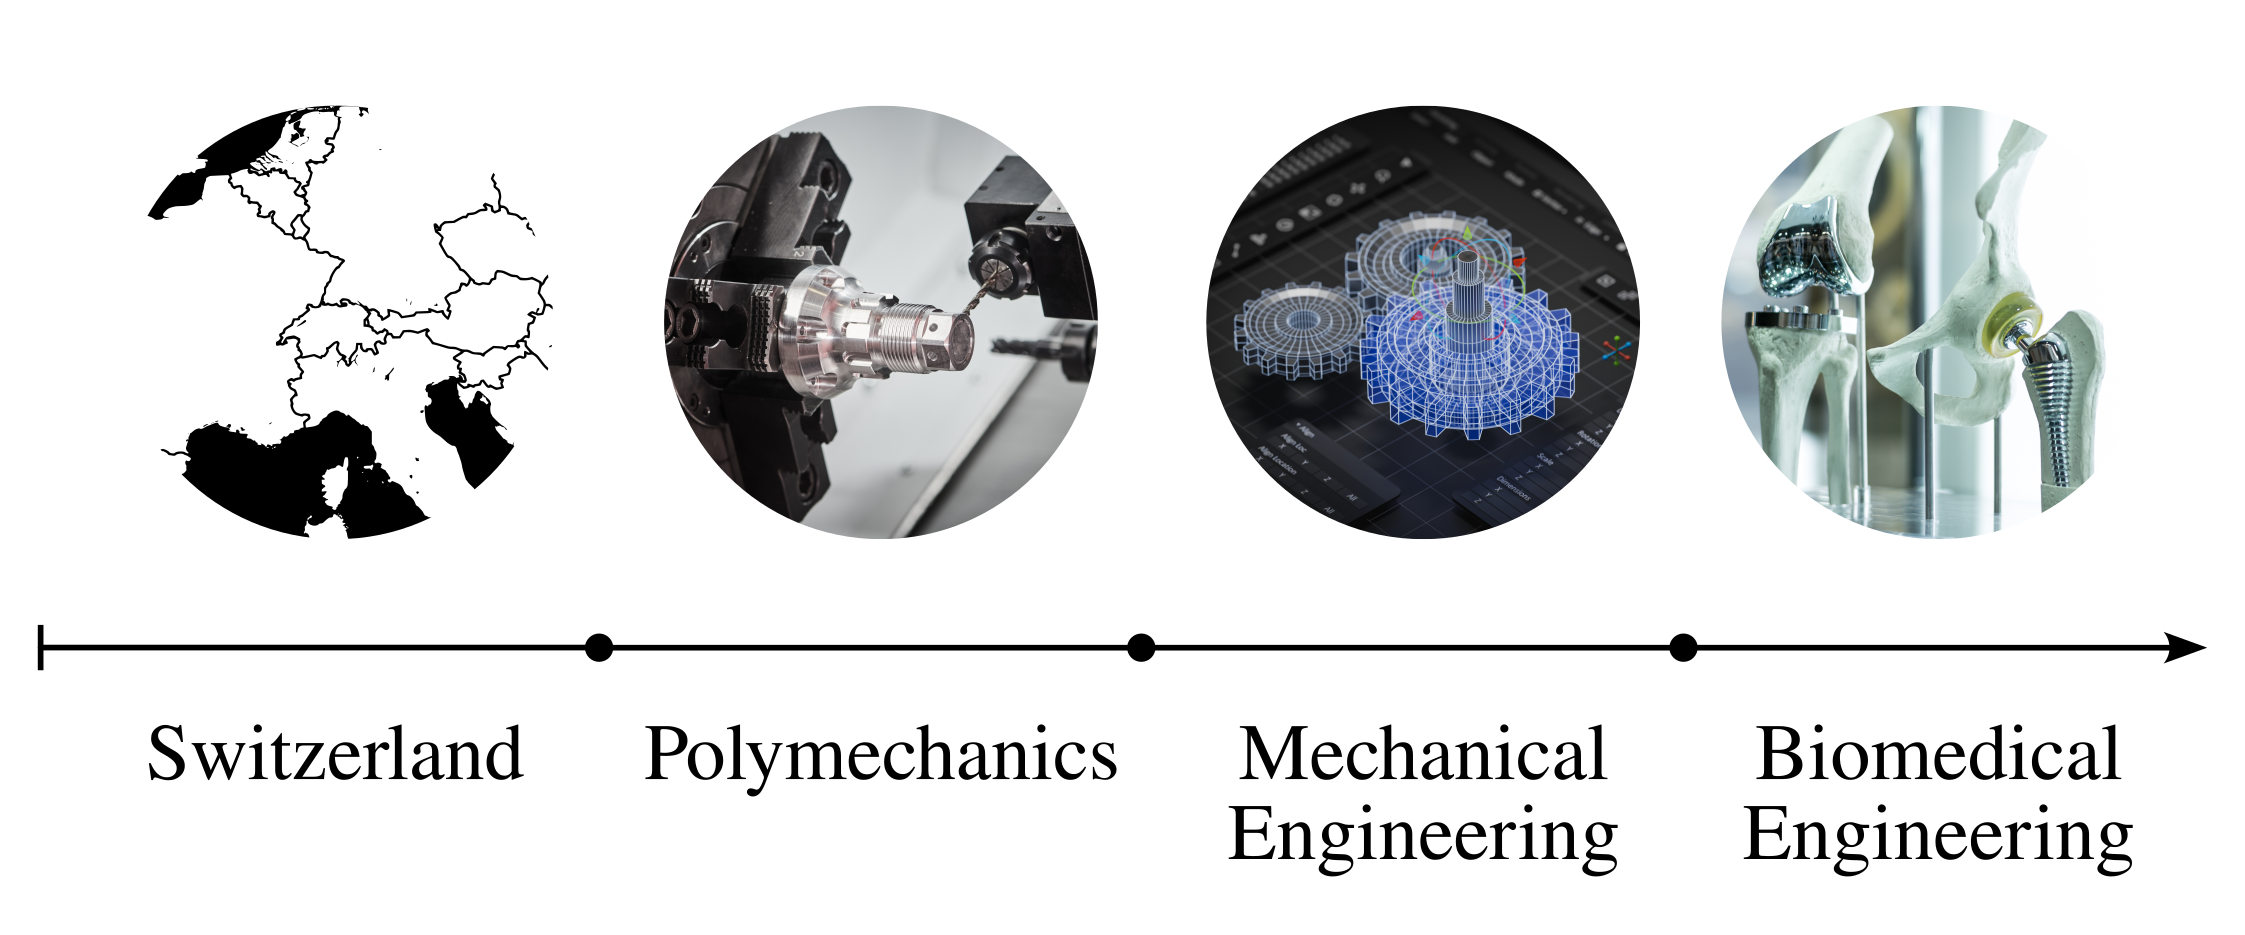
\includegraphics[width=\linewidth]{Figures/Journey}
	\end{frame}

	\begin{frame}
			\frametitle{Thesis and Postdoc}
			\begin{columns}
					\column{0.45\linewidth}
					PhD Main Aspects
					\begin{enumerate}
							\item Finite Element Analysis
							\item Experimental Validation
							\item Image Segmentation and Analysis
					\end{enumerate}
					\vspace{5mm}
					Postdoc\\
					Aortic Dissection Risk from Intramural Structure
					\column{0.50\linewidth}
					\centering
					\begin{figure}
					\tcbox[colframe=black,colback=white,boxsep=0px,boxrule=0.25mm,sharp corners=all,leftrule=3mm]{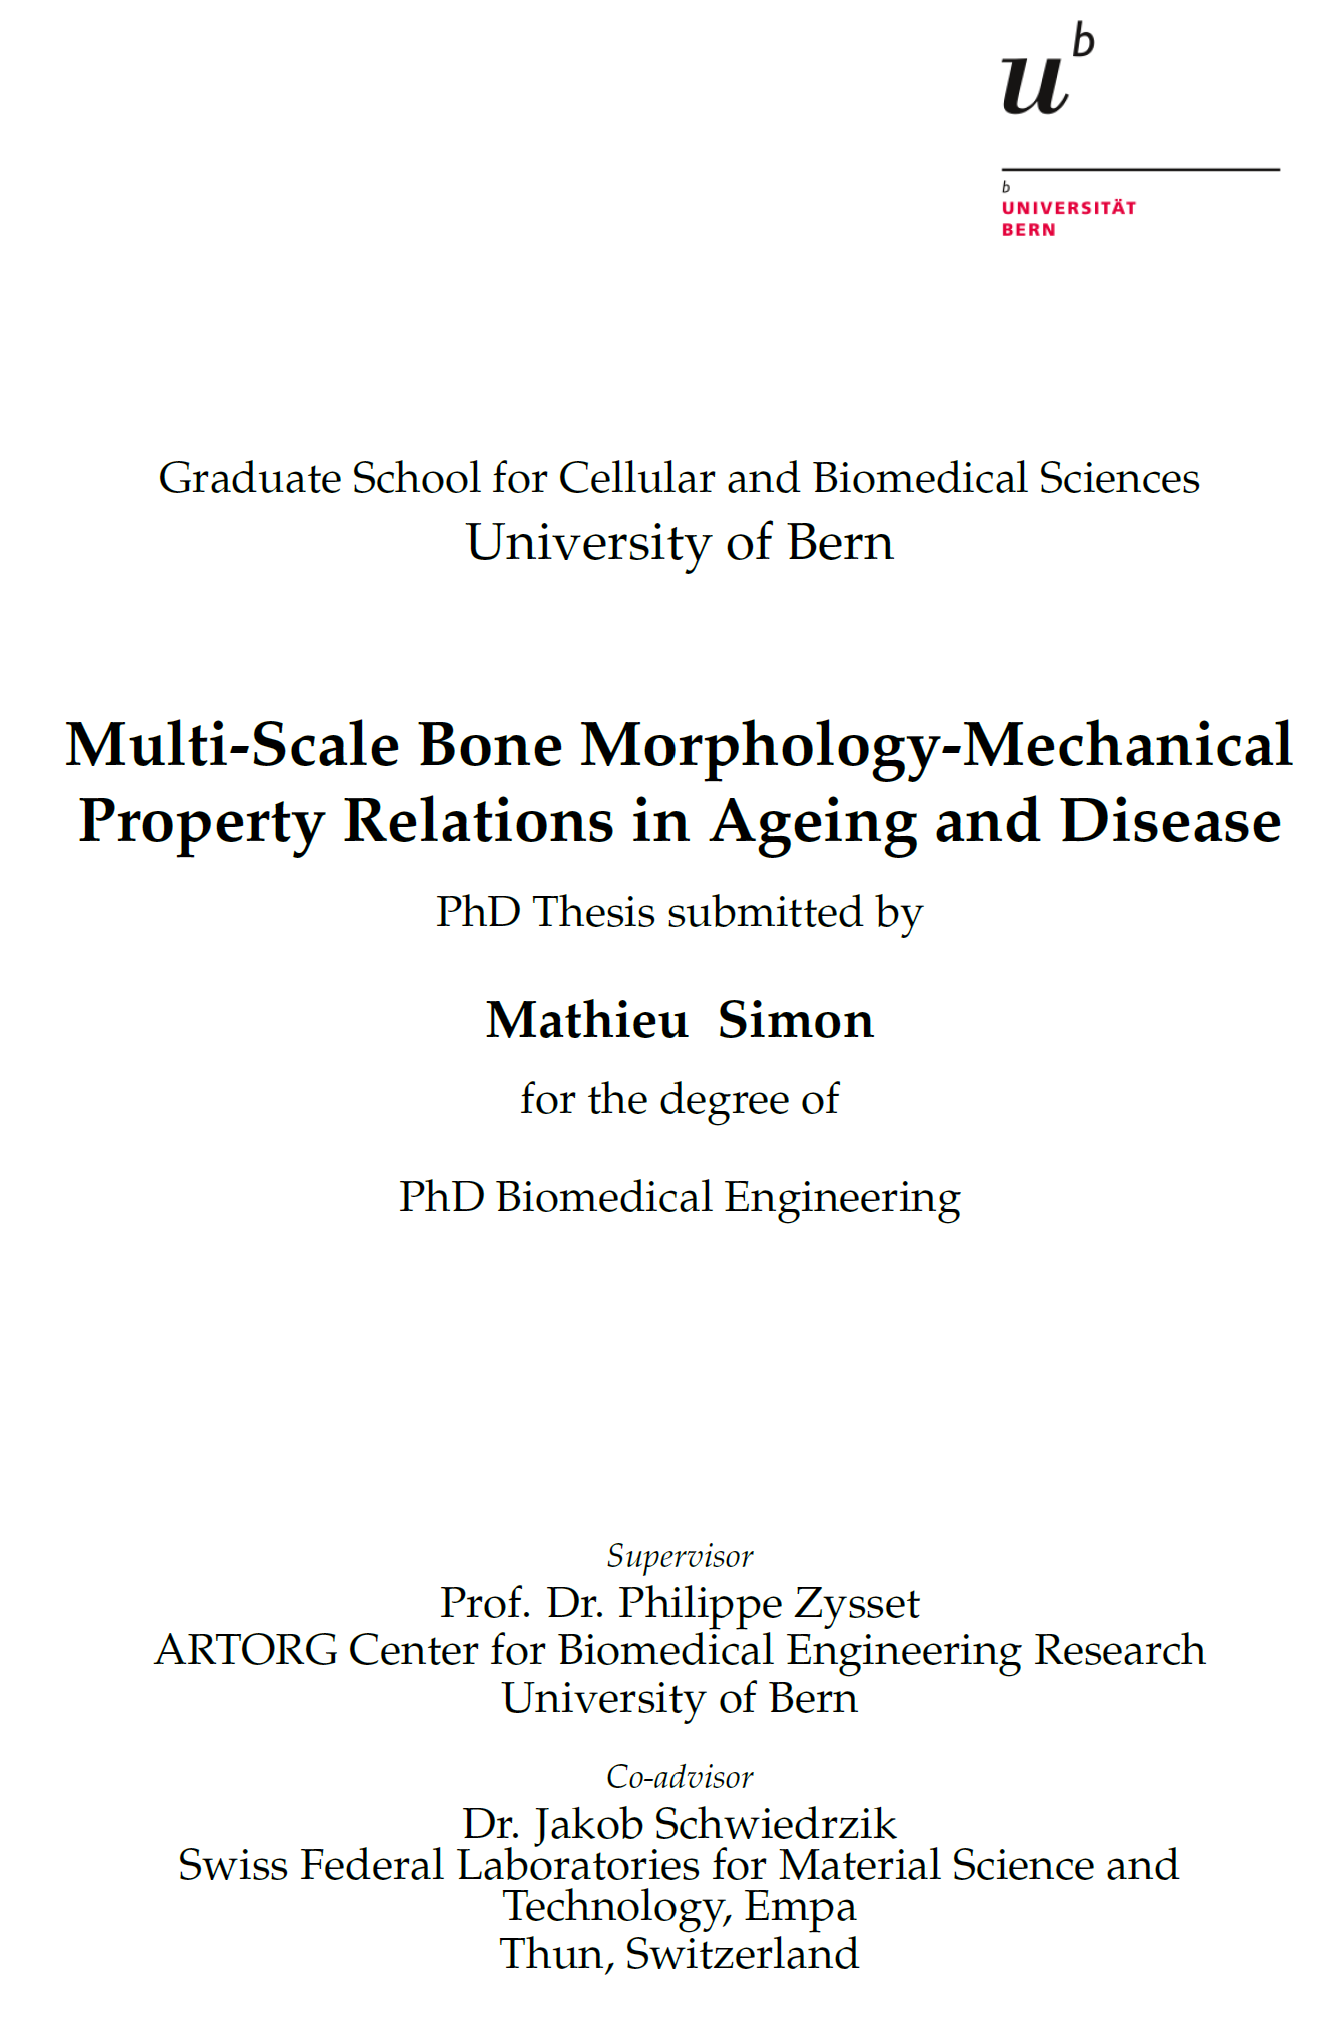
\includegraphics[width=0.6\linewidth]{Figures/PhDTitle}}
					\end{figure}
			\end{columns}
	\end{frame}

	%----------------------------------------------------------------
	%----------------------------------------------------------------
	%----------------------------------------------------------------
	
	\section{Introduction}

	% \begin{frame}
	% 	\frametitle{Bone}
	% 	\framesubtitle{Anatomy}
	% 	\begin{columns}
	% 		\column{0.42\linewidth}
	% 		Cortical bone
	% 		\begin{itemize}
	% 			\item Outer shell
	% 			\item Dense\\85-95\% volume fraction
	% 			\item Pore size about 0.1 mm
	% 		\end{itemize}
	% 		\vspace{5mm}
	% 		Trabecular bone
	% 		\begin{itemize}
	% 			\item Internal network
	% 			\item Porous\\5-45\% volume fraction
	% 			\item Pore size about 1 mm
	% 		\end{itemize}
	% 		\column{0.55\linewidth}
	% 		\centering
	% 		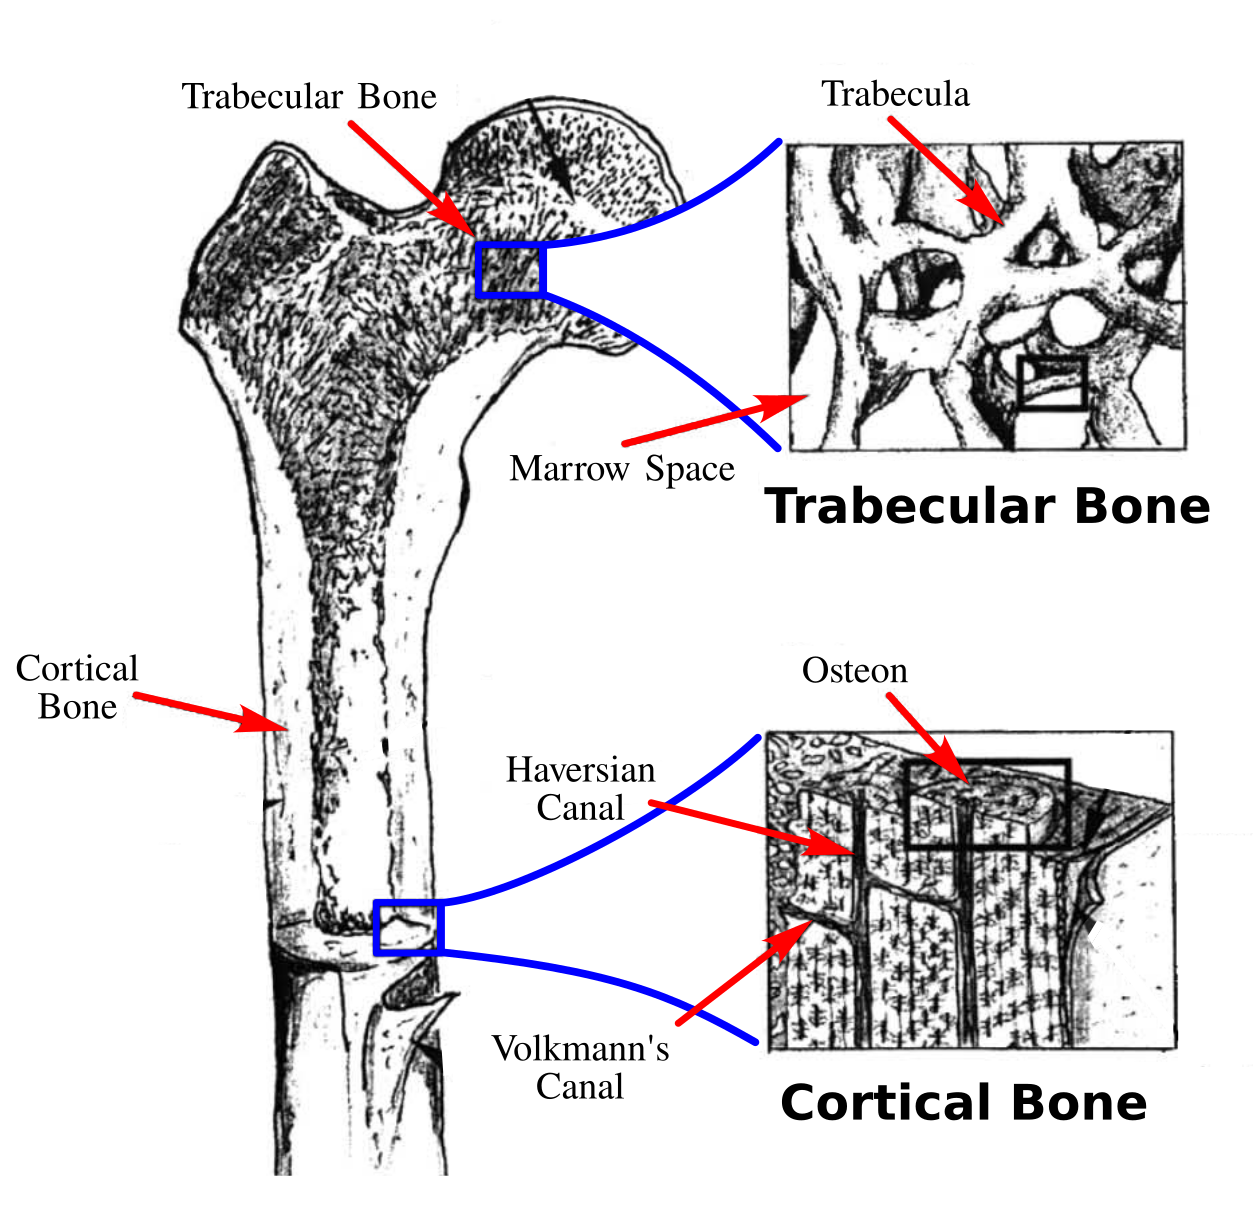
\includegraphics[width=\linewidth]{Figures/Bone.png}
	% 	\end{columns}
	% \end{frame}

	% \begin{frame}
	% 	\frametitle{Bone}
	% 	\framesubtitle{Functions}
	% 	\begin{columns}
	% 		\column{0.42\linewidth}
	% 		Bone organ involved in:
	% 		\begin{itemize}
	% 			\item Mechanical support
	% 			\item Organs protection
	% 			\item Haematopoesis
	% 			\item Calcium Homeostasis
	% 		\end{itemize}
	% 		\vspace{5mm}
	% 		Mechanical adaptation
	% 		\begin{itemize}
	% 			\item Modeling and remodeling
	% 			\item Mechanostat theory
	% 		\end{itemize}
	% 		\column{0.55\linewidth}
	% 		\centering
	% 		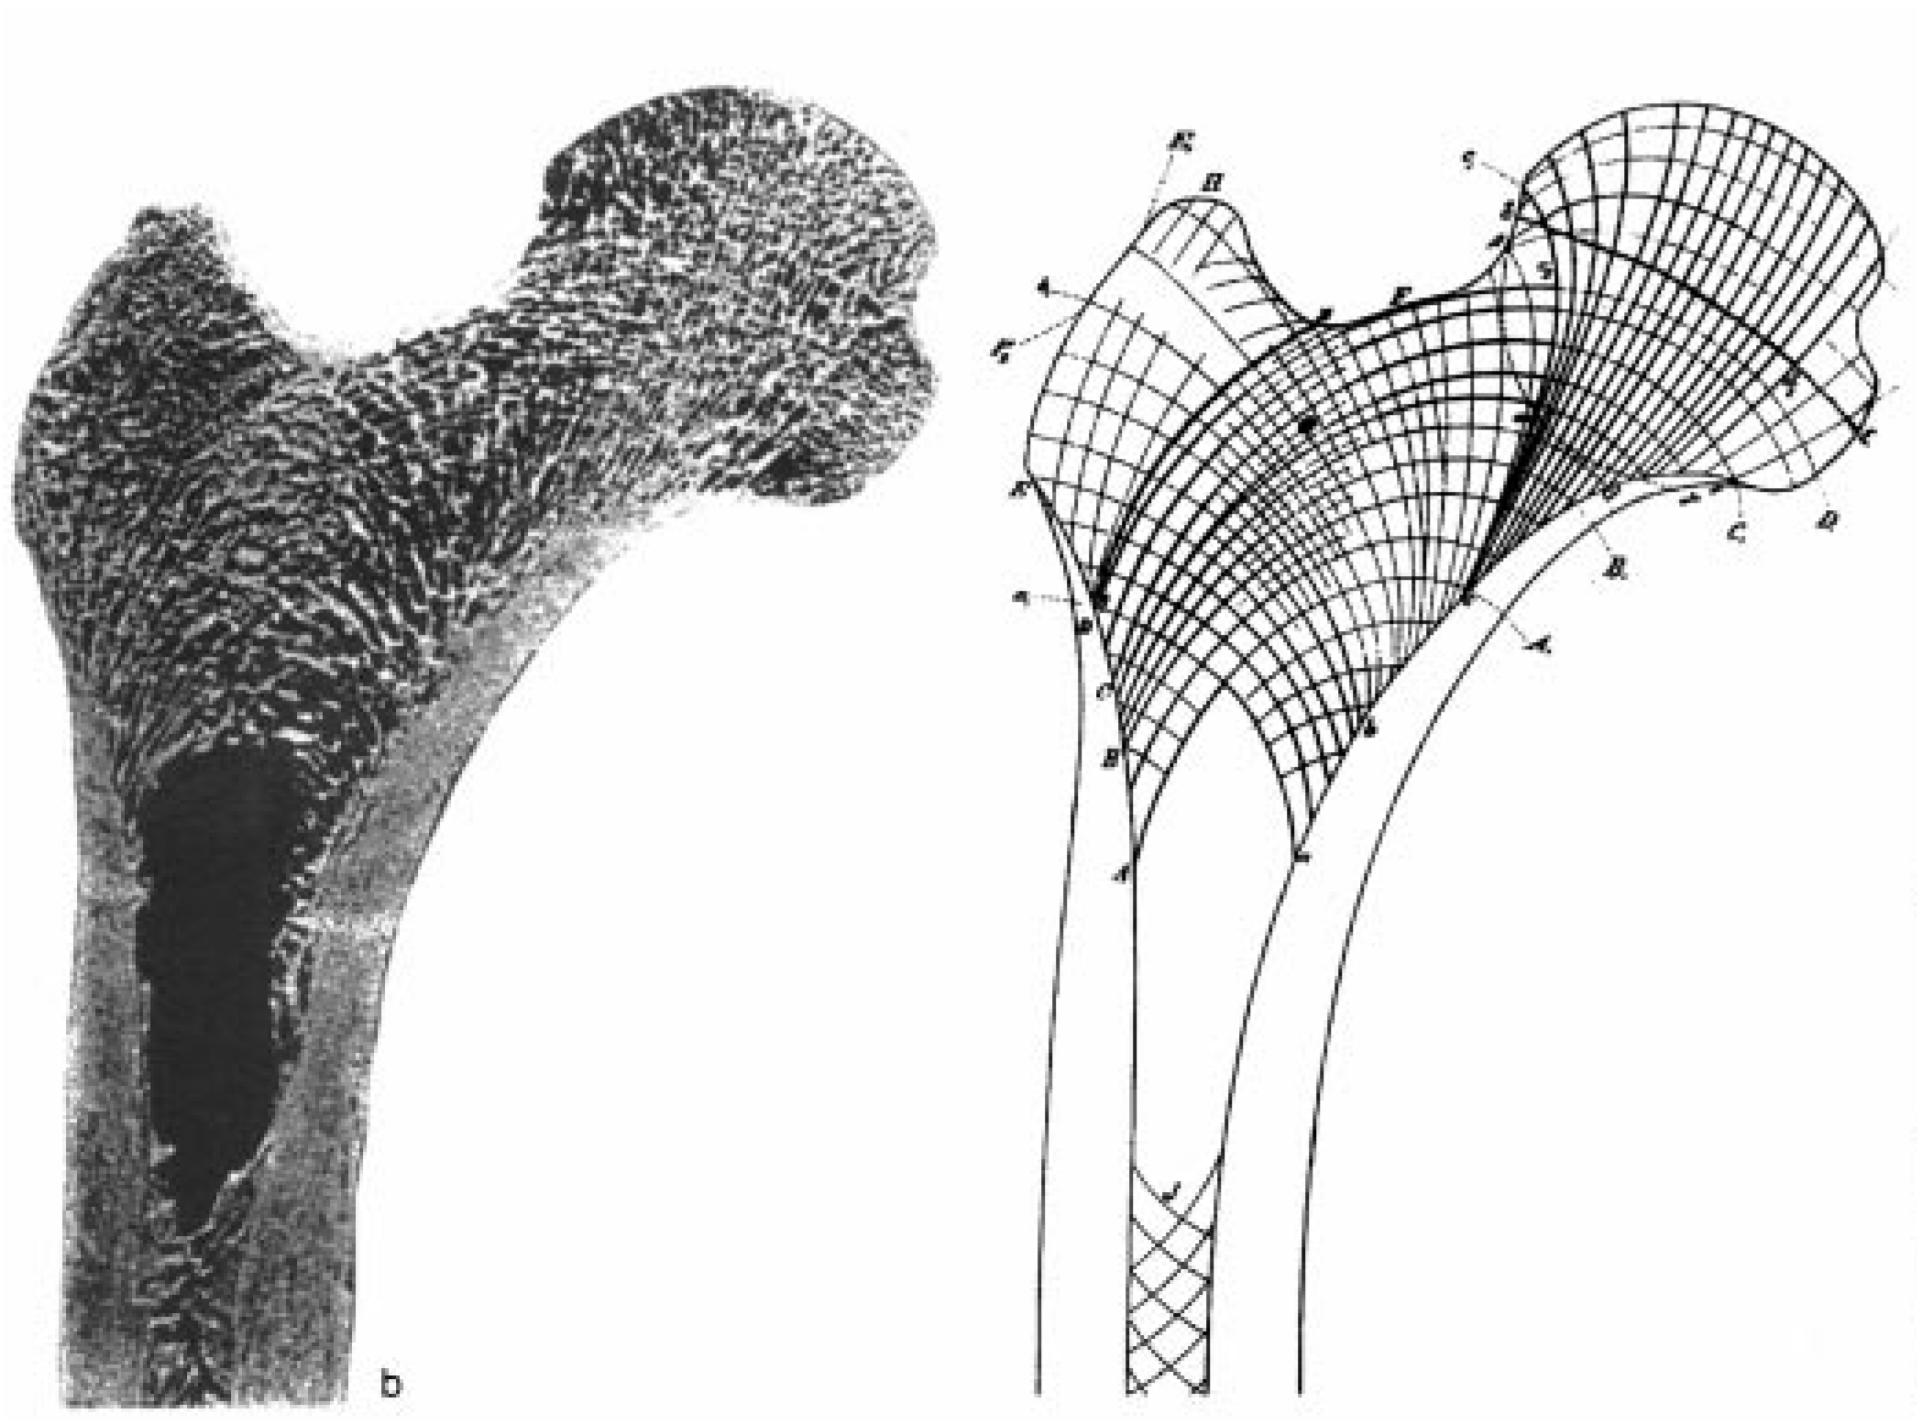
\includegraphics[width=\linewidth]{Figures/MeyerAndCulmann_Cropped.png}
	% 	\end{columns}
	% \end{frame}

	\begin{frame}
		\frametitle{Bone}
		\framesubtitle{Ageing and Disease}
		\begin{columns}
			\column[t]{0.475\linewidth}
			Ageing
			\begin{itemize}
				\item Loss of bone mass
				\item Increased fracture risk
			\end{itemize}
			\vspace{5mm}
			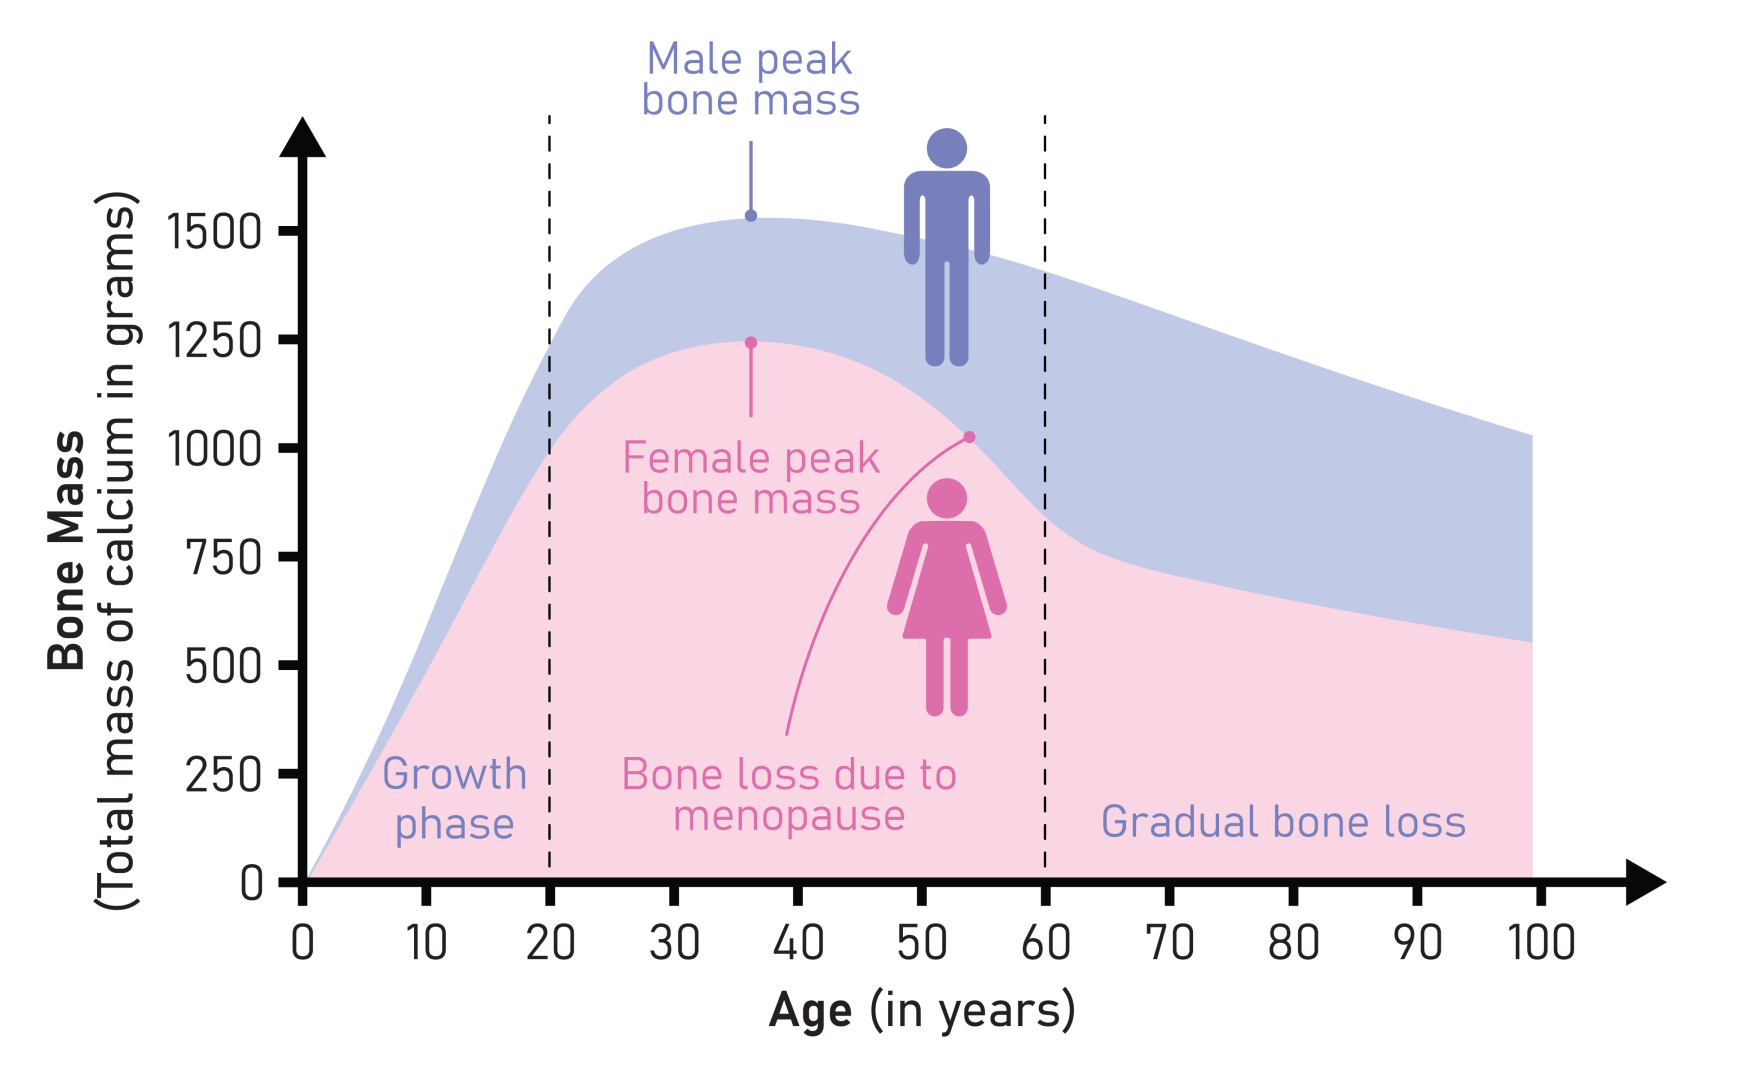
\includegraphics[width=\linewidth]{Figures/BoneMass.png}
			\column[t]{0.475\linewidth}
			Fragility fractures
			\begin{itemize}
				\item Occurs every 3\textsuperscript{rd} second
				\item Treatment gap: about 70\%
			\end{itemize}
			\vspace{8mm}
			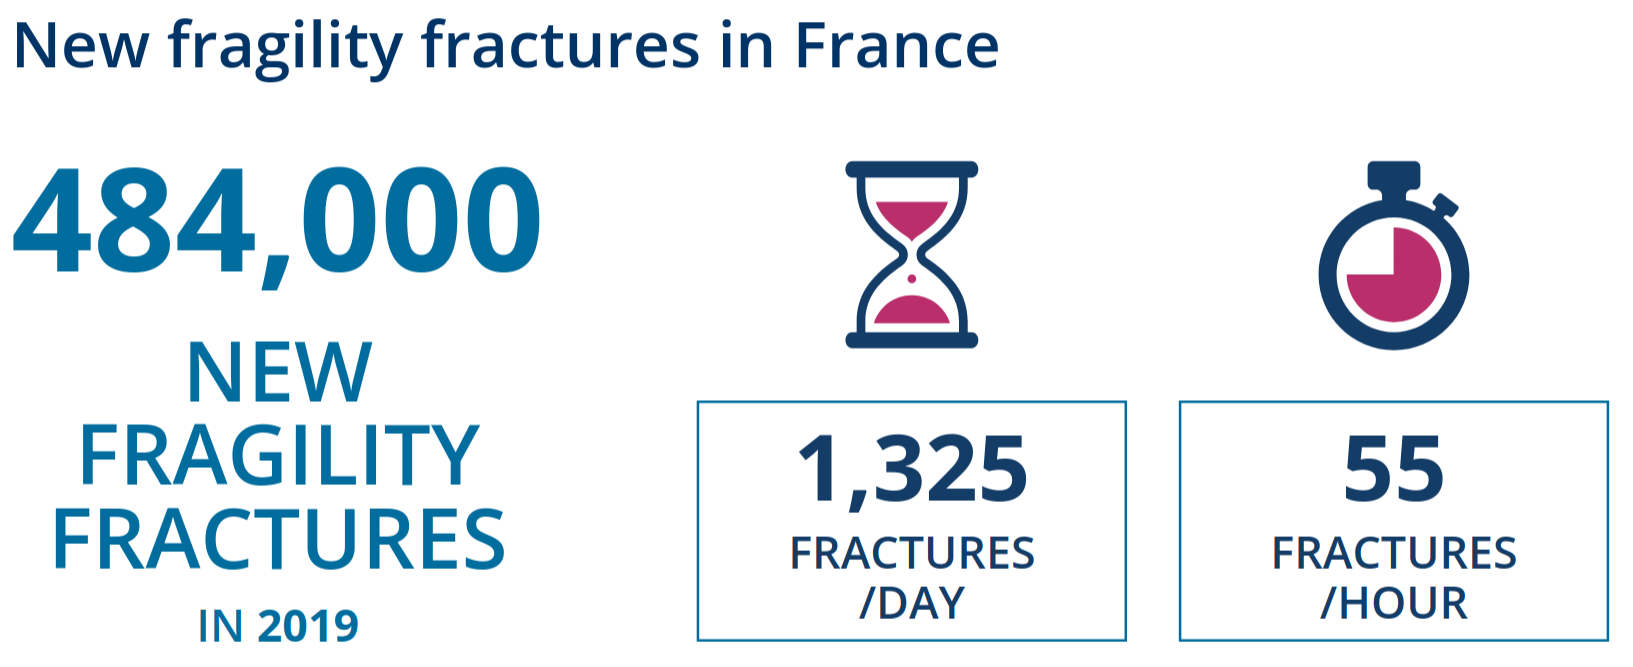
\includegraphics[width=\linewidth]{Figures/France.png}
		\end{columns}
		\vfill
		\hfill\Tiny{Kanis et al. (2021)}
	\end{frame}

	\begin{frame}
		\frametitle{Bone}
		\framesubtitle{Imaging}
		\begin{columns}
			\column{0.5\linewidth}
			HR-pQCT
			\begin{itemize}
				\item \textbf{H}igh \textbf{R}esolution:\\72 – 61 \textmu m
				\item \textbf{P}eripheral:\\Radius or tibia
				\item \textbf{Q}uantitative:\\Bone mineral density (BMD)
				\item \textbf{C}omputed \textbf{T}omography:\\3D bone structure
			\end{itemize}
			\column{0.45\linewidth}
			\centering
			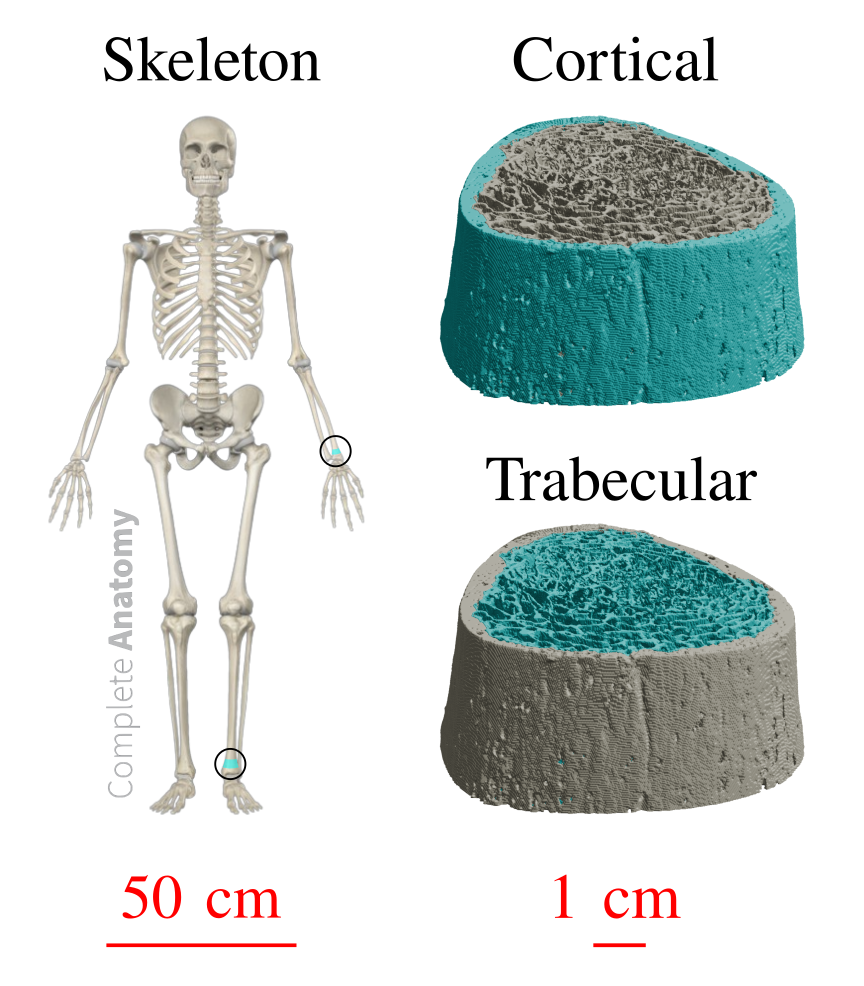
\includegraphics[width=\linewidth]{Figures/HR-pQCT.png}
		\end{columns}
	\end{frame}

	\begin{frame}
		\frametitle{Finite Element Analysis}
		\begin{columns}
			\column{0.65\linewidth}
			Micro-Finite Element (\textmu FE)
			\begin{itemize}
				\item Accurate geometry representation
				\item High computational costs
			\end{itemize}
			\vspace{5mm}
			Homogenized Finite Element (hFE)
			\begin{itemize}
				\item Structural properties of a larger region\\Bone volume fraction and fabric
				\item Significantly lower computational costs
				\item Accurate prediction of bone properties\textsuperscript{1}
			\end{itemize}
			\column{0.3\linewidth}
			\centering
			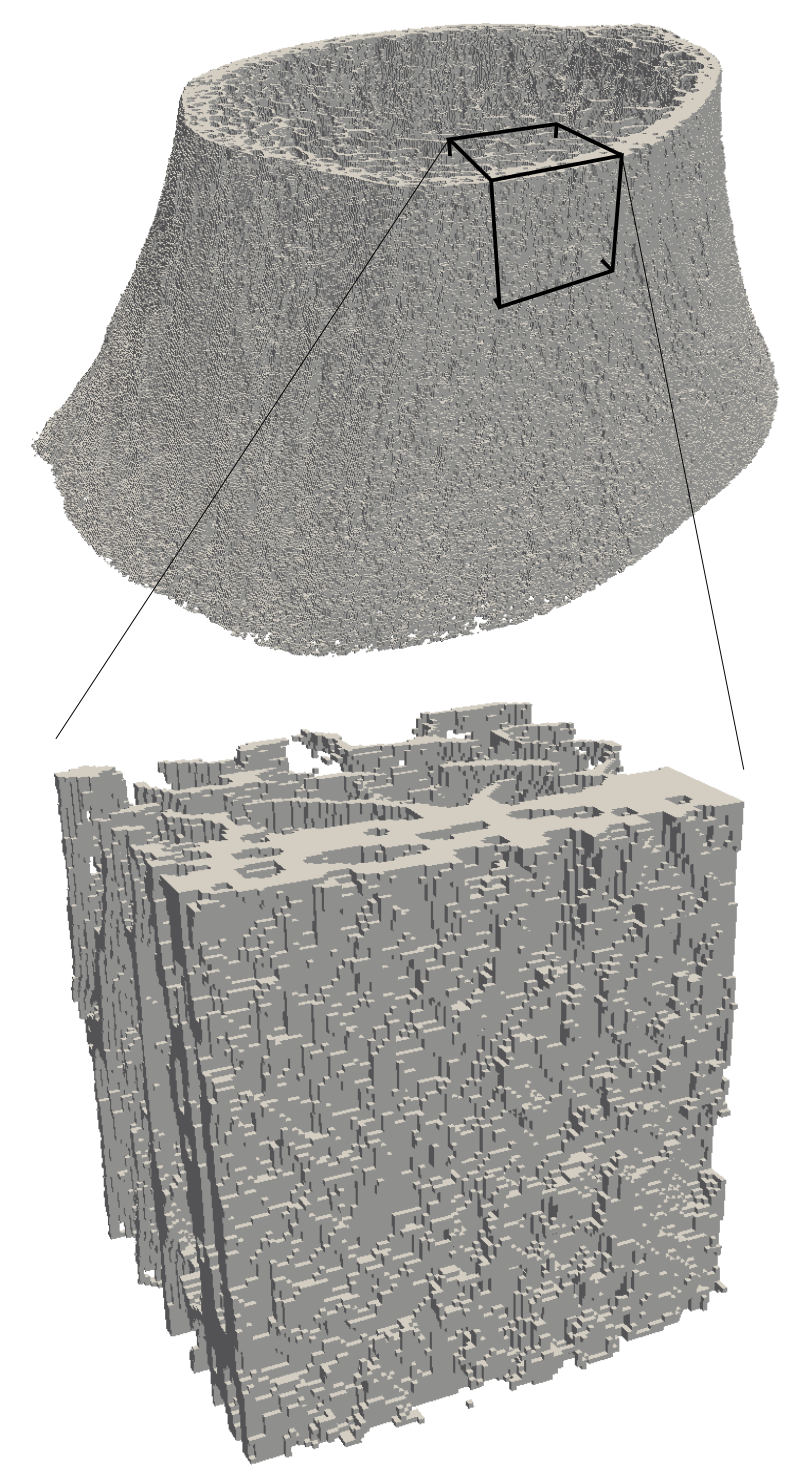
\includegraphics[width=\linewidth]{Figures/HighResCT.png}
		\end{columns}
		\vfill
		\hfill\Tiny{\textsuperscript{1}Schenk et al. (2022)}
	\end{frame}

	\begin{frame}
		\frametitle{Research Objectives}

		\begin{columns}
			\column{0.65\linewidth}
			HR-pQCT of distal radius \ding{51}

			\vspace{1cm}

			HR-pQCT of distal tibia
			\begin{itemize}
				\item Mechanical data set
				\item Validation of hFE analysis
				\begin{itemize}
					\item Structural properties
					\item Strain localization
				\end{itemize}
			\end{itemize}

			\column{0.30\linewidth}
			\centering
			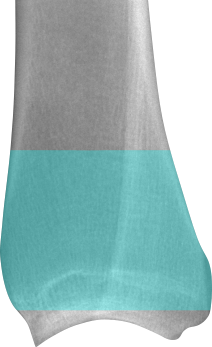
\includegraphics[height=0.9\linewidth]{Figures/Clinic}\\
			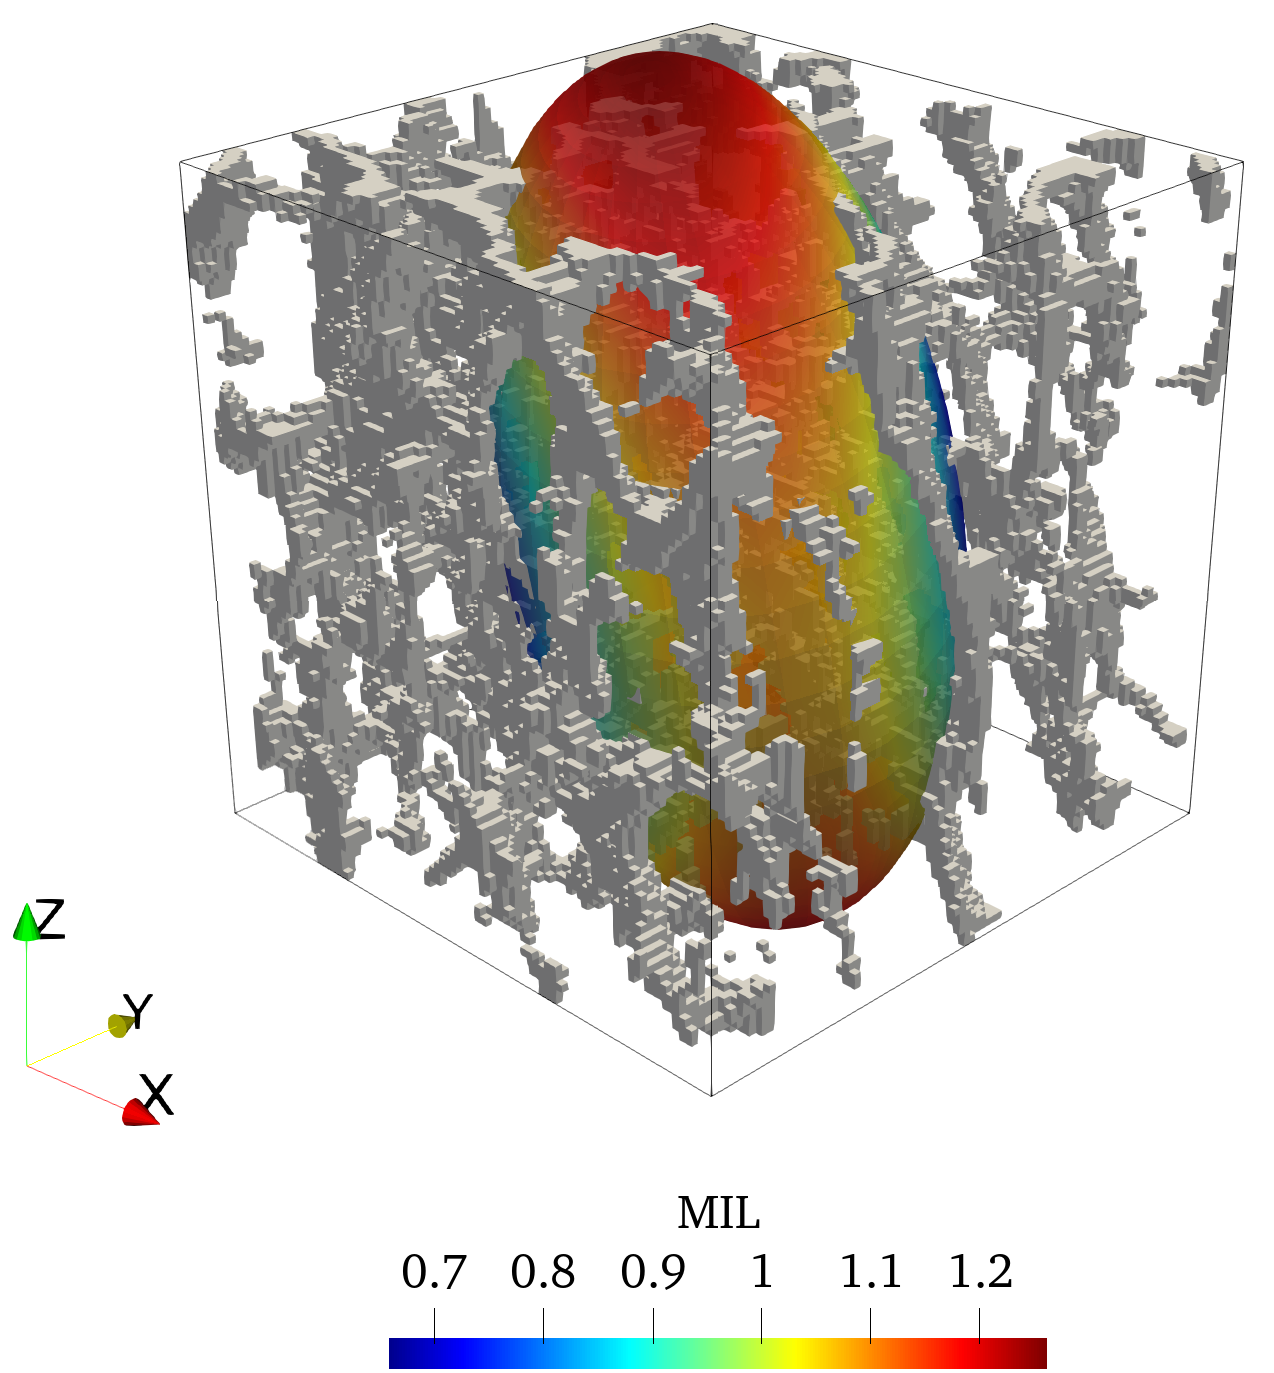
\includegraphics[width=0.9\linewidth]{Figures/Fabric}

		\end{columns}

	\end{frame}

	% %----------------------------------------------------------------
	% %----------------------------------------------------------------
	% %----------------------------------------------------------------
	
	\section{Methods}

	\begin{frame}
		\frametitle{Material and Methods}
		\framesubtitle{Fresh Frozen Samples}
		\centering
		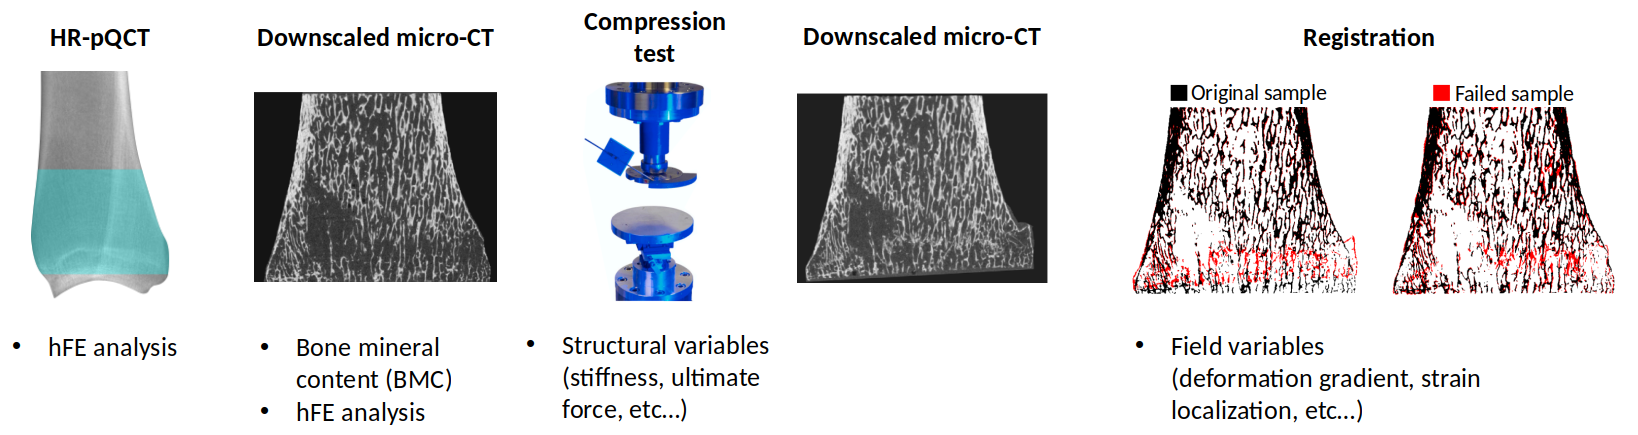
\includegraphics[width=1.0\linewidth]{Figures/MethodsFull1}
	\end{frame}

	\begin{frame}
		\frametitle{Analysis}
		\begin{columns}
			\column{0.5\linewidth}
			Linear Regression
			\begin{itemize}
				\item HR-pQCT vs \textmu CT
				\item BMC vs Structural Variables
				\item hFE vs Structural Variables
			\end{itemize}
			\vspace{5mm}
			Qualitative Comparison
			\begin{itemize}
				\item hFE vs Registration
			\end{itemize}

			\column{0.5\linewidth}
			\centering
			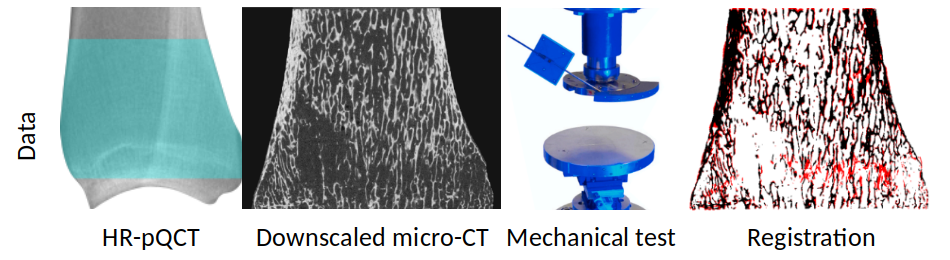
\includegraphics[width=1.0\linewidth, trim=20 0 20 0]{Figures/MethodsFull2a}\\
			\vspace{5mm}
			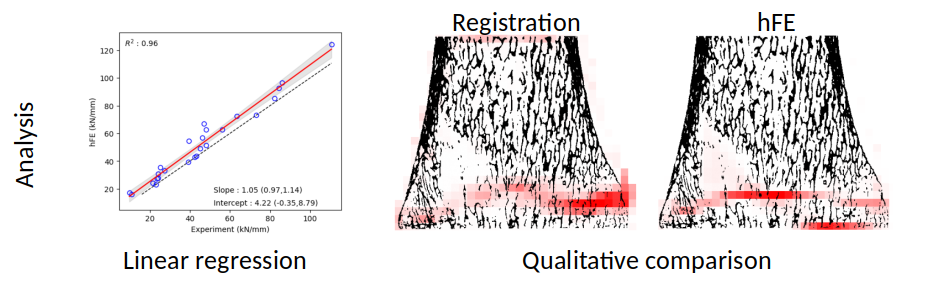
\includegraphics[width=1.0\linewidth, trim=20 0 20 0]{Figures/MethodsFull2b}
		\end{columns}

	\end{frame}

	% \begin{frame}
	% 	\frametitle{Sample Set}
	% 	25 samples - University of Vienna, Vienna, Austria\\
	% 	\vfill
	% 	\centering
	% 	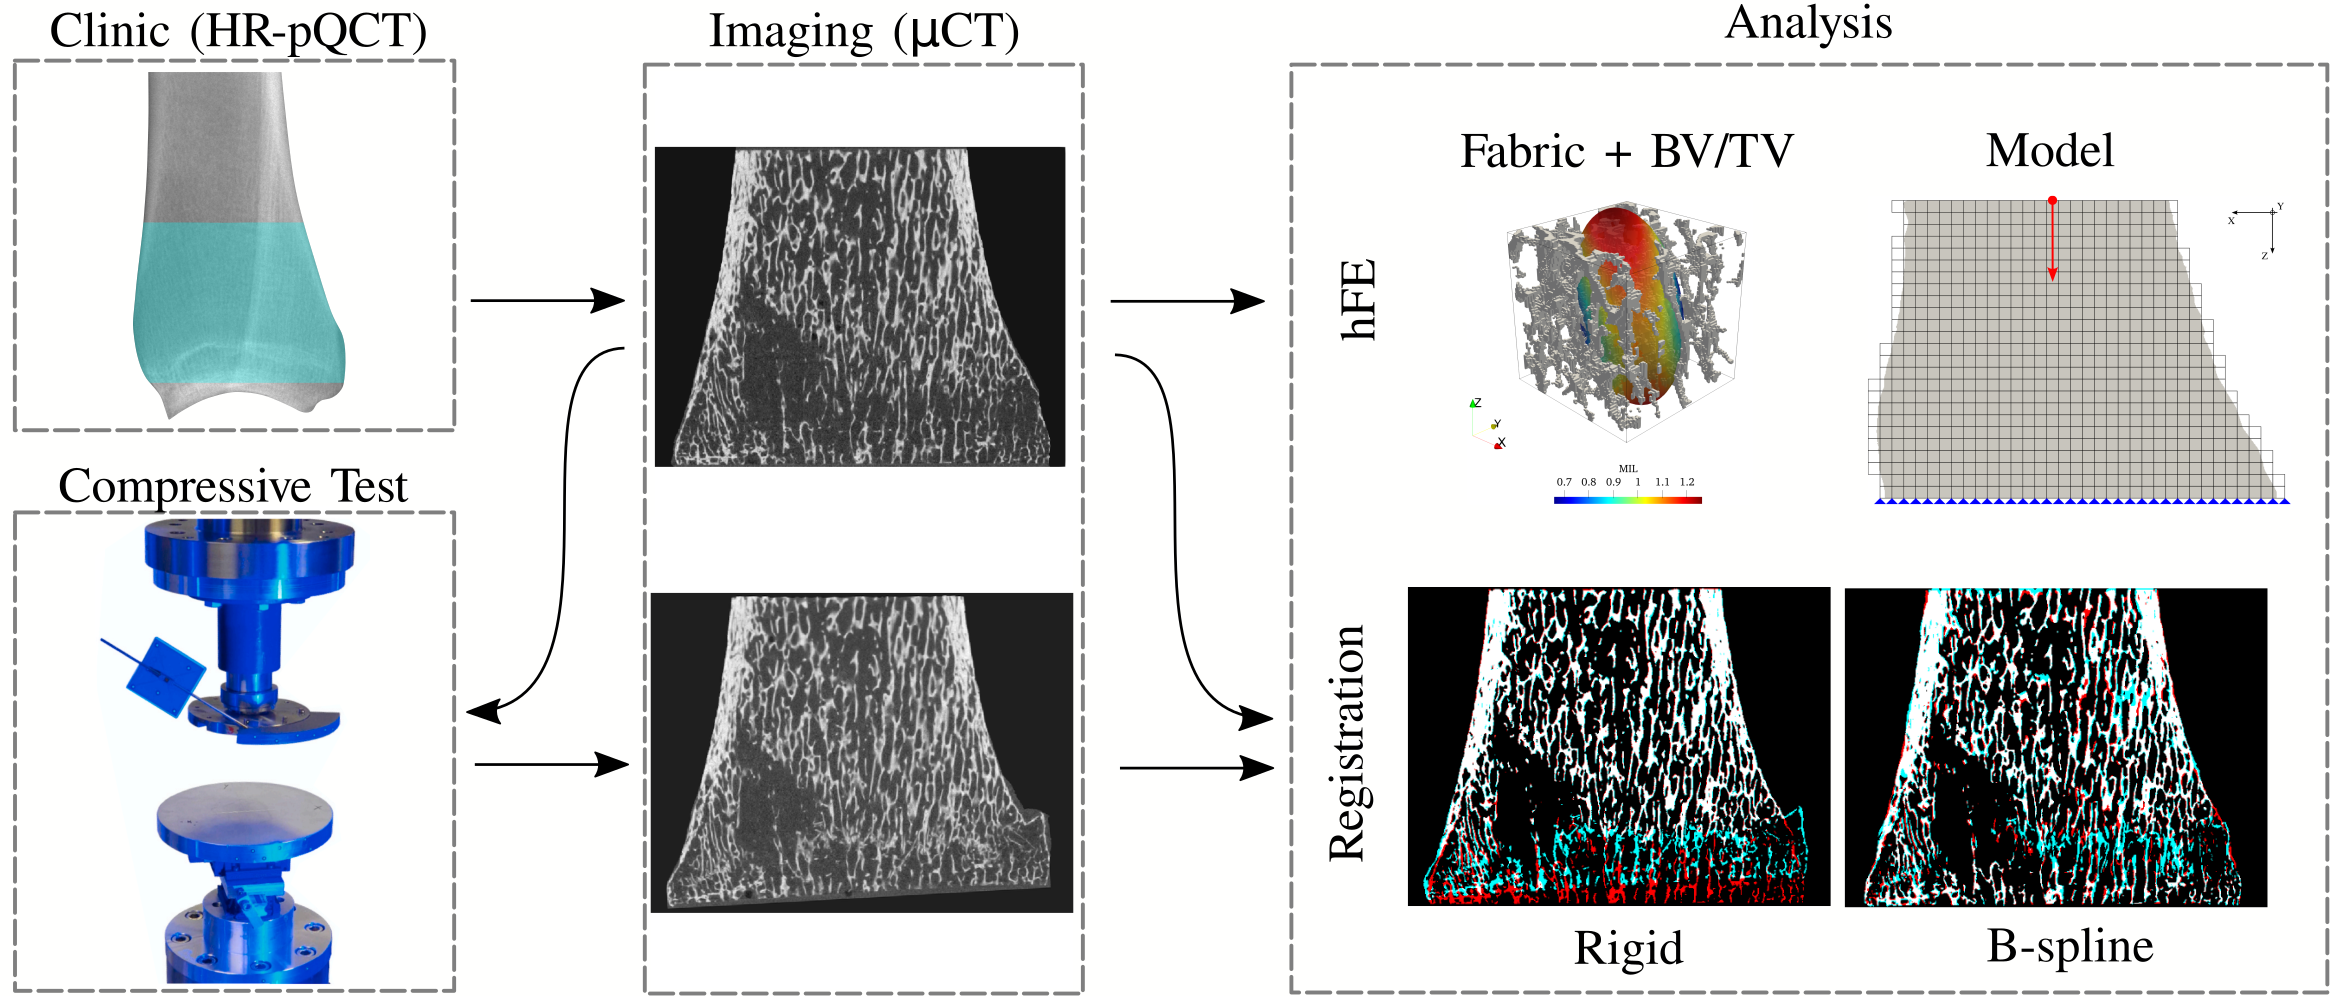
\includegraphics[width=1.0\linewidth]{Figures/Methods}
	% \end{frame}

	% \begin{frame}[noframenumbering]
	% 	\frametitle{HR-pQCT Scan}
	% 	Morphometry and hFE\\
	% 	\vfill
	% 	\centering
	% 	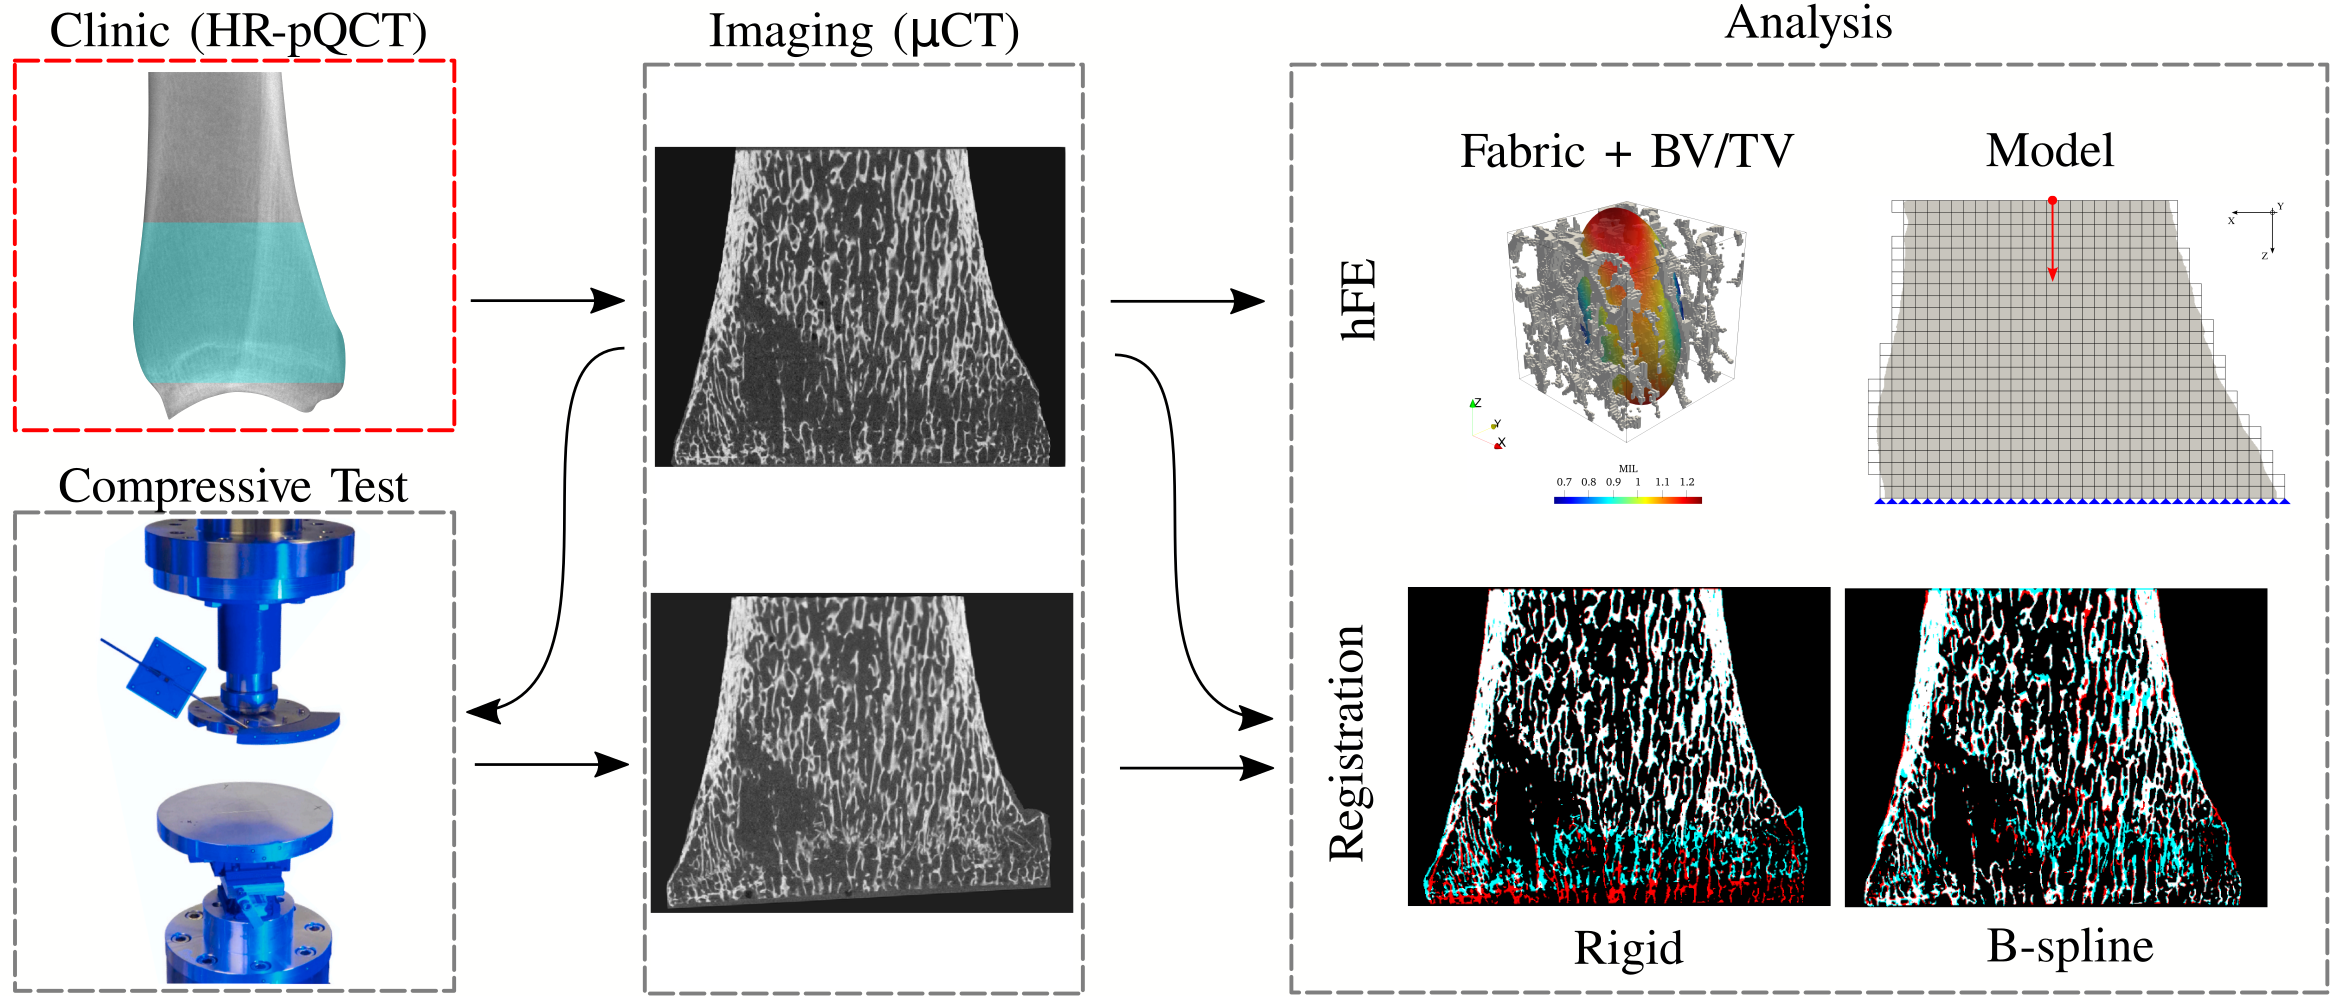
\includegraphics[width=1.0\linewidth]{Figures/Methods1}
	% \end{frame}

	% \begin{frame}[noframenumbering]
	% 	\frametitle{High-Resolution MicroCT Scan}
	% 	Morphometry and densitometry\\
	% 	\vfill
	% 	\centering
	% 	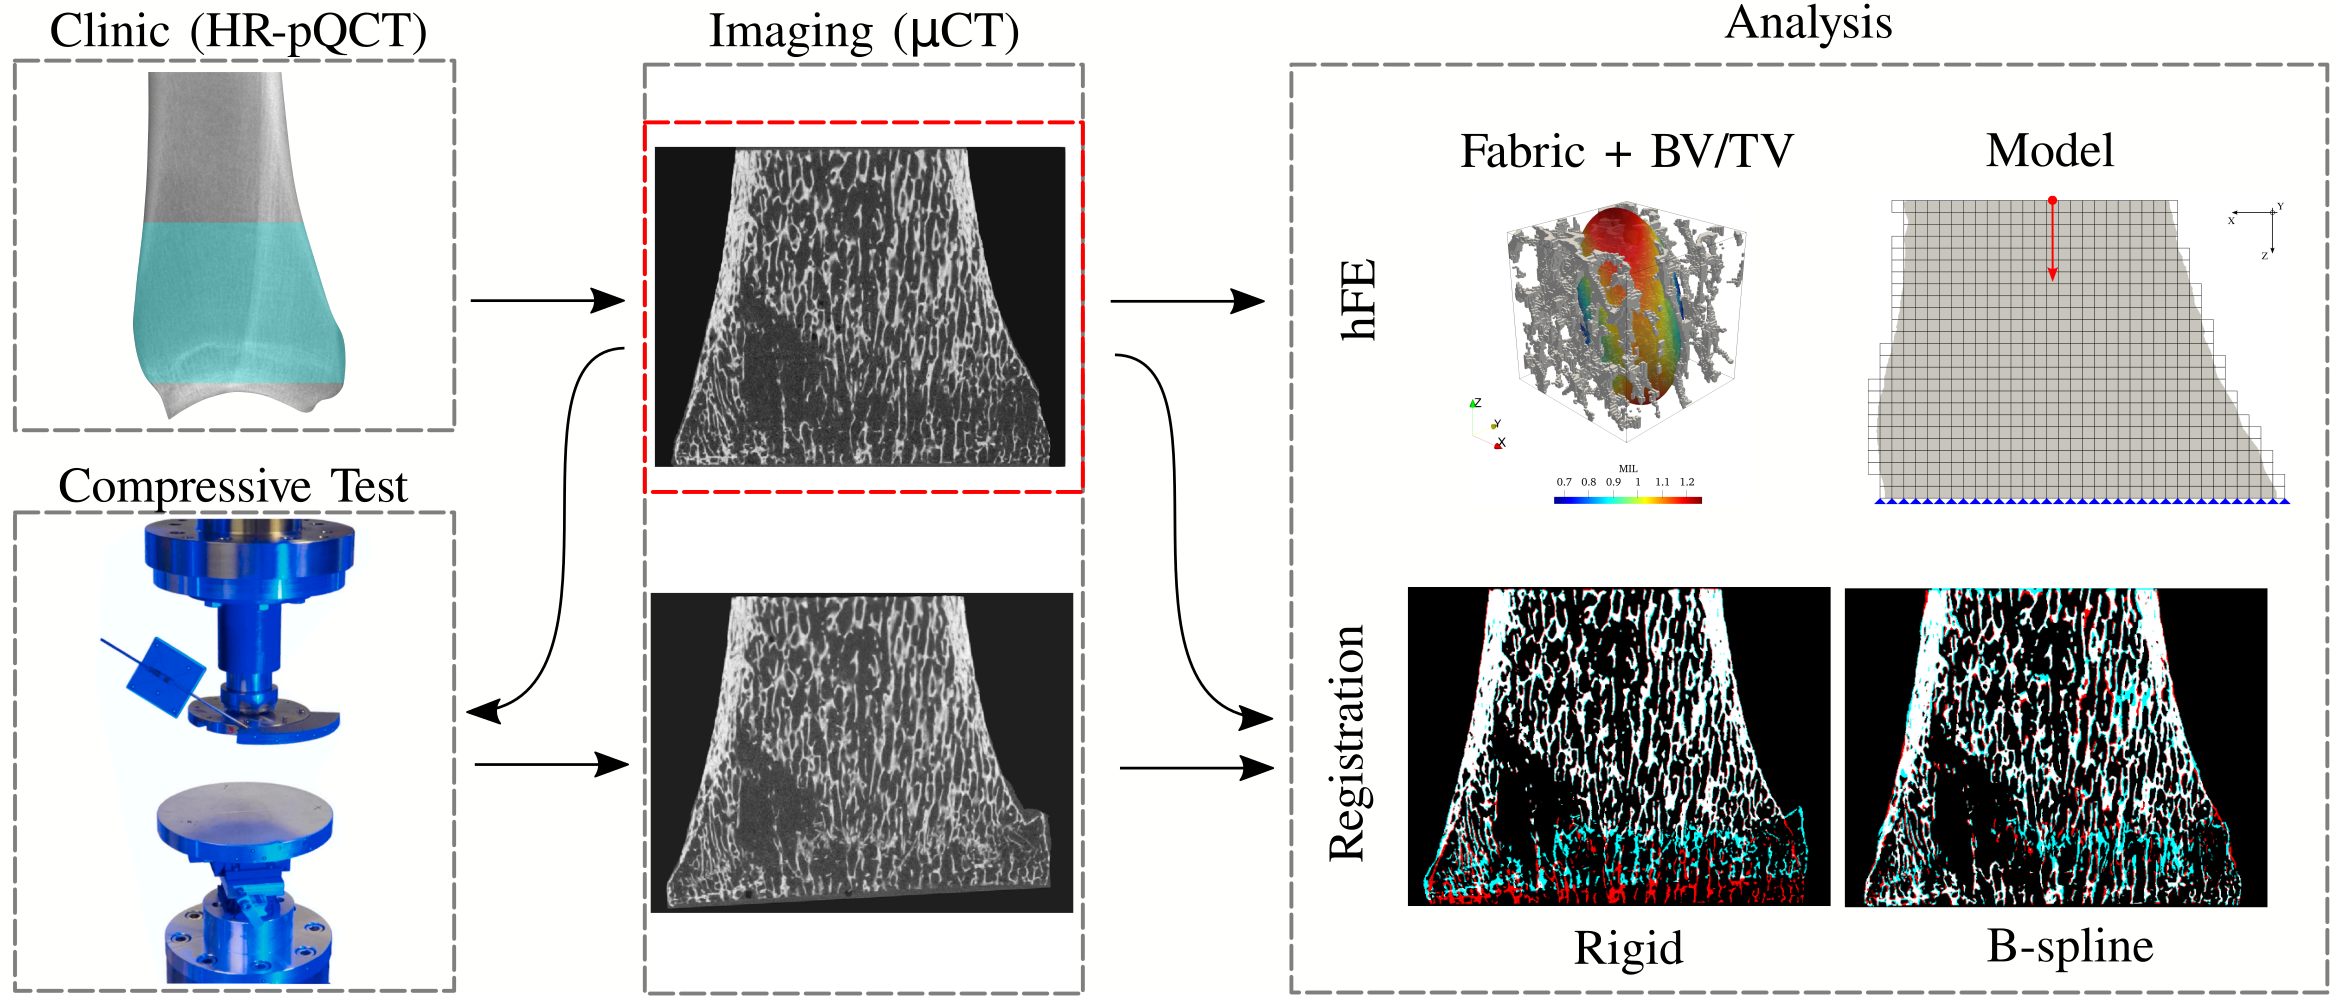
\includegraphics[width=1.0\linewidth]{Figures/Methods2}
	% \end{frame}

	% \begin{frame}[noframenumbering]
	% 	\frametitle{Experimental Tests}
	% 	Mechanical properties - AO Institute, Davos, Switzerland\\
	% 	\vfill
	% 	\centering
	% 	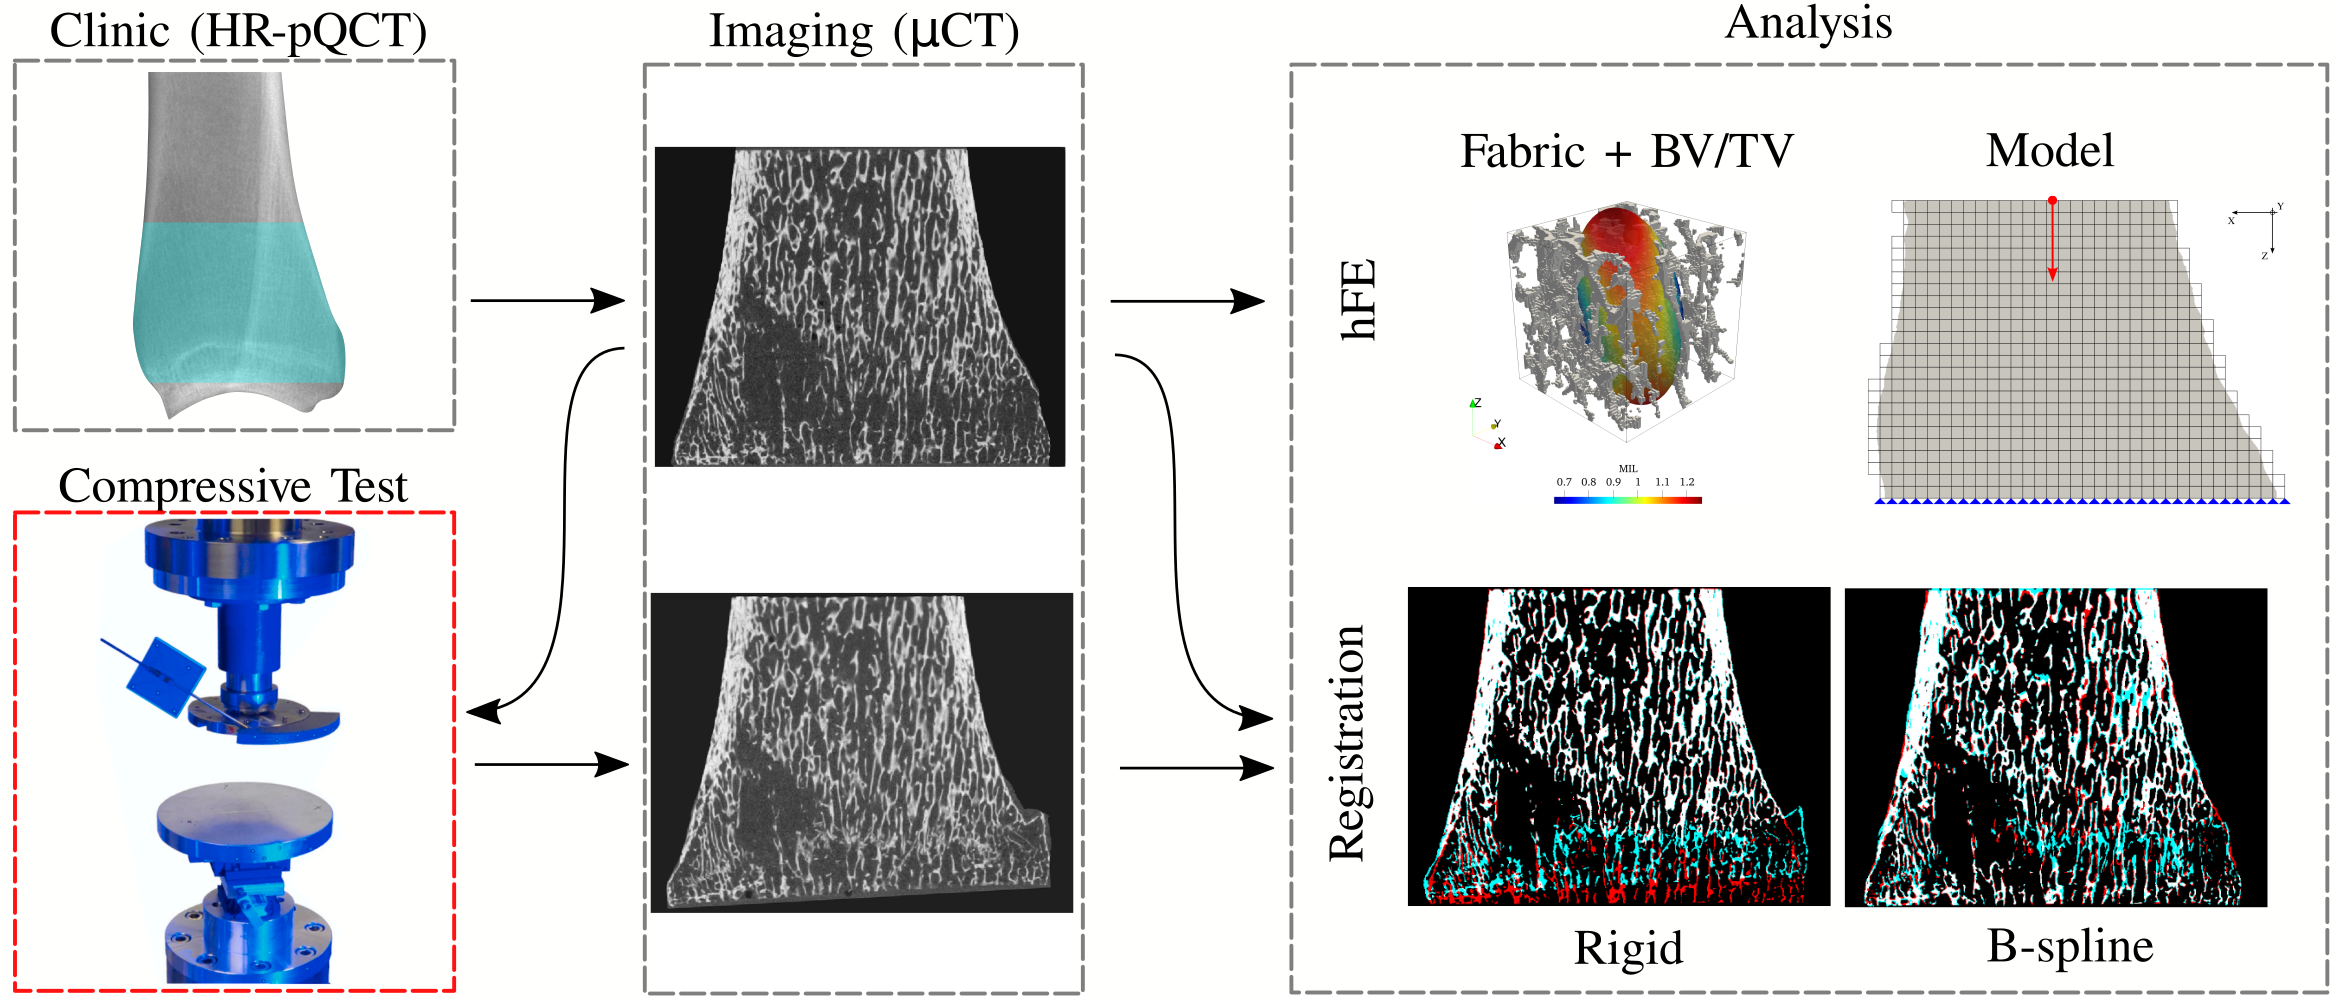
\includegraphics[width=1.0\linewidth]{Figures/Methods3}
	% \end{frame}

	% \begin{frame}[noframenumbering]
	% 	\frametitle{Experimental Tests}
	% 	Mechanical properties - data set characterization\\
	% 	\vfill
	% 	\centering
	% 	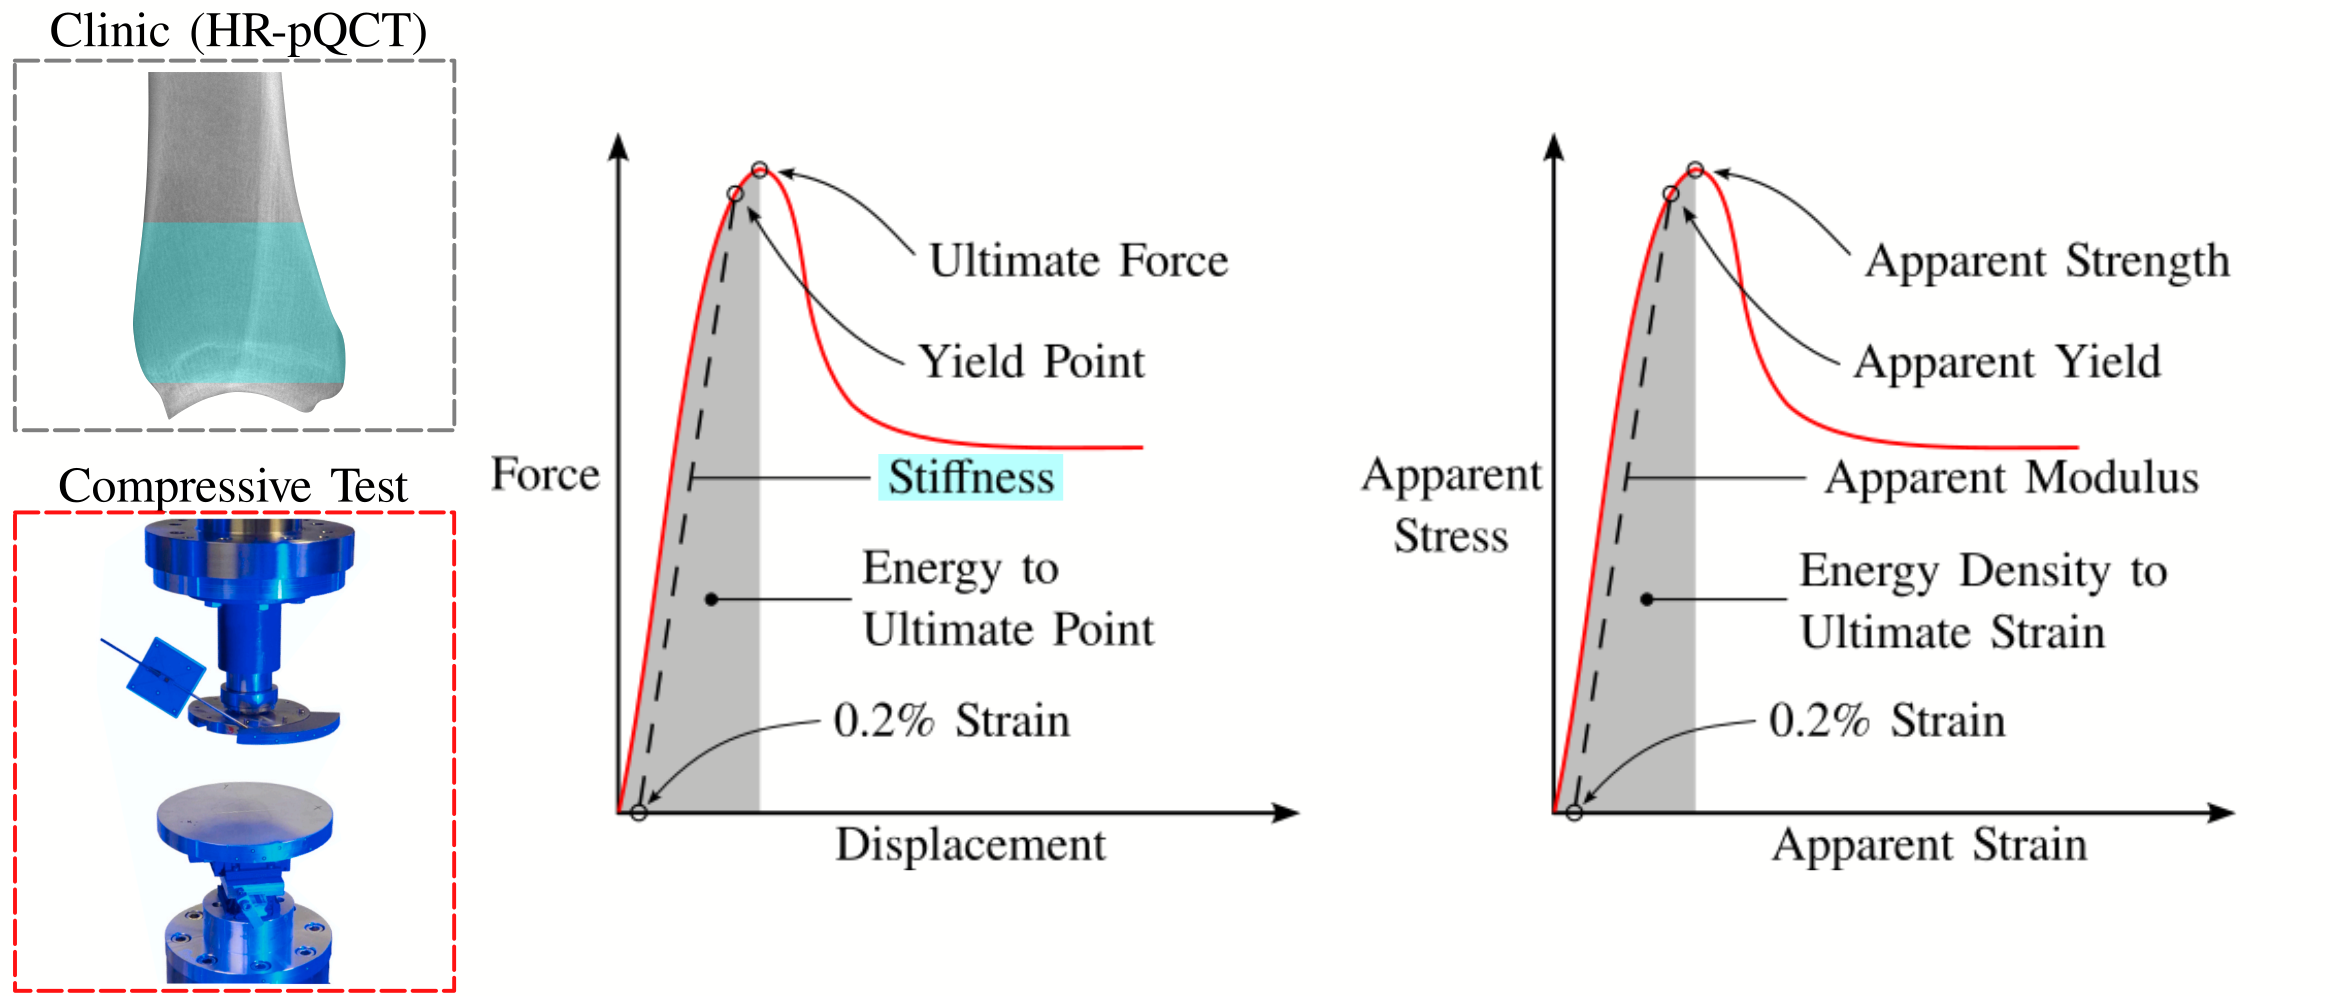
\includegraphics[width=1.0\linewidth]{Figures/Methods3b}
	% \end{frame}

	% \begin{frame}[noframenumbering]
	% 	\frametitle{High-Resolution MicroCT Scan}
	% 	Failed configuration\\
	% 	\vfill
	% 	\centering
	% 	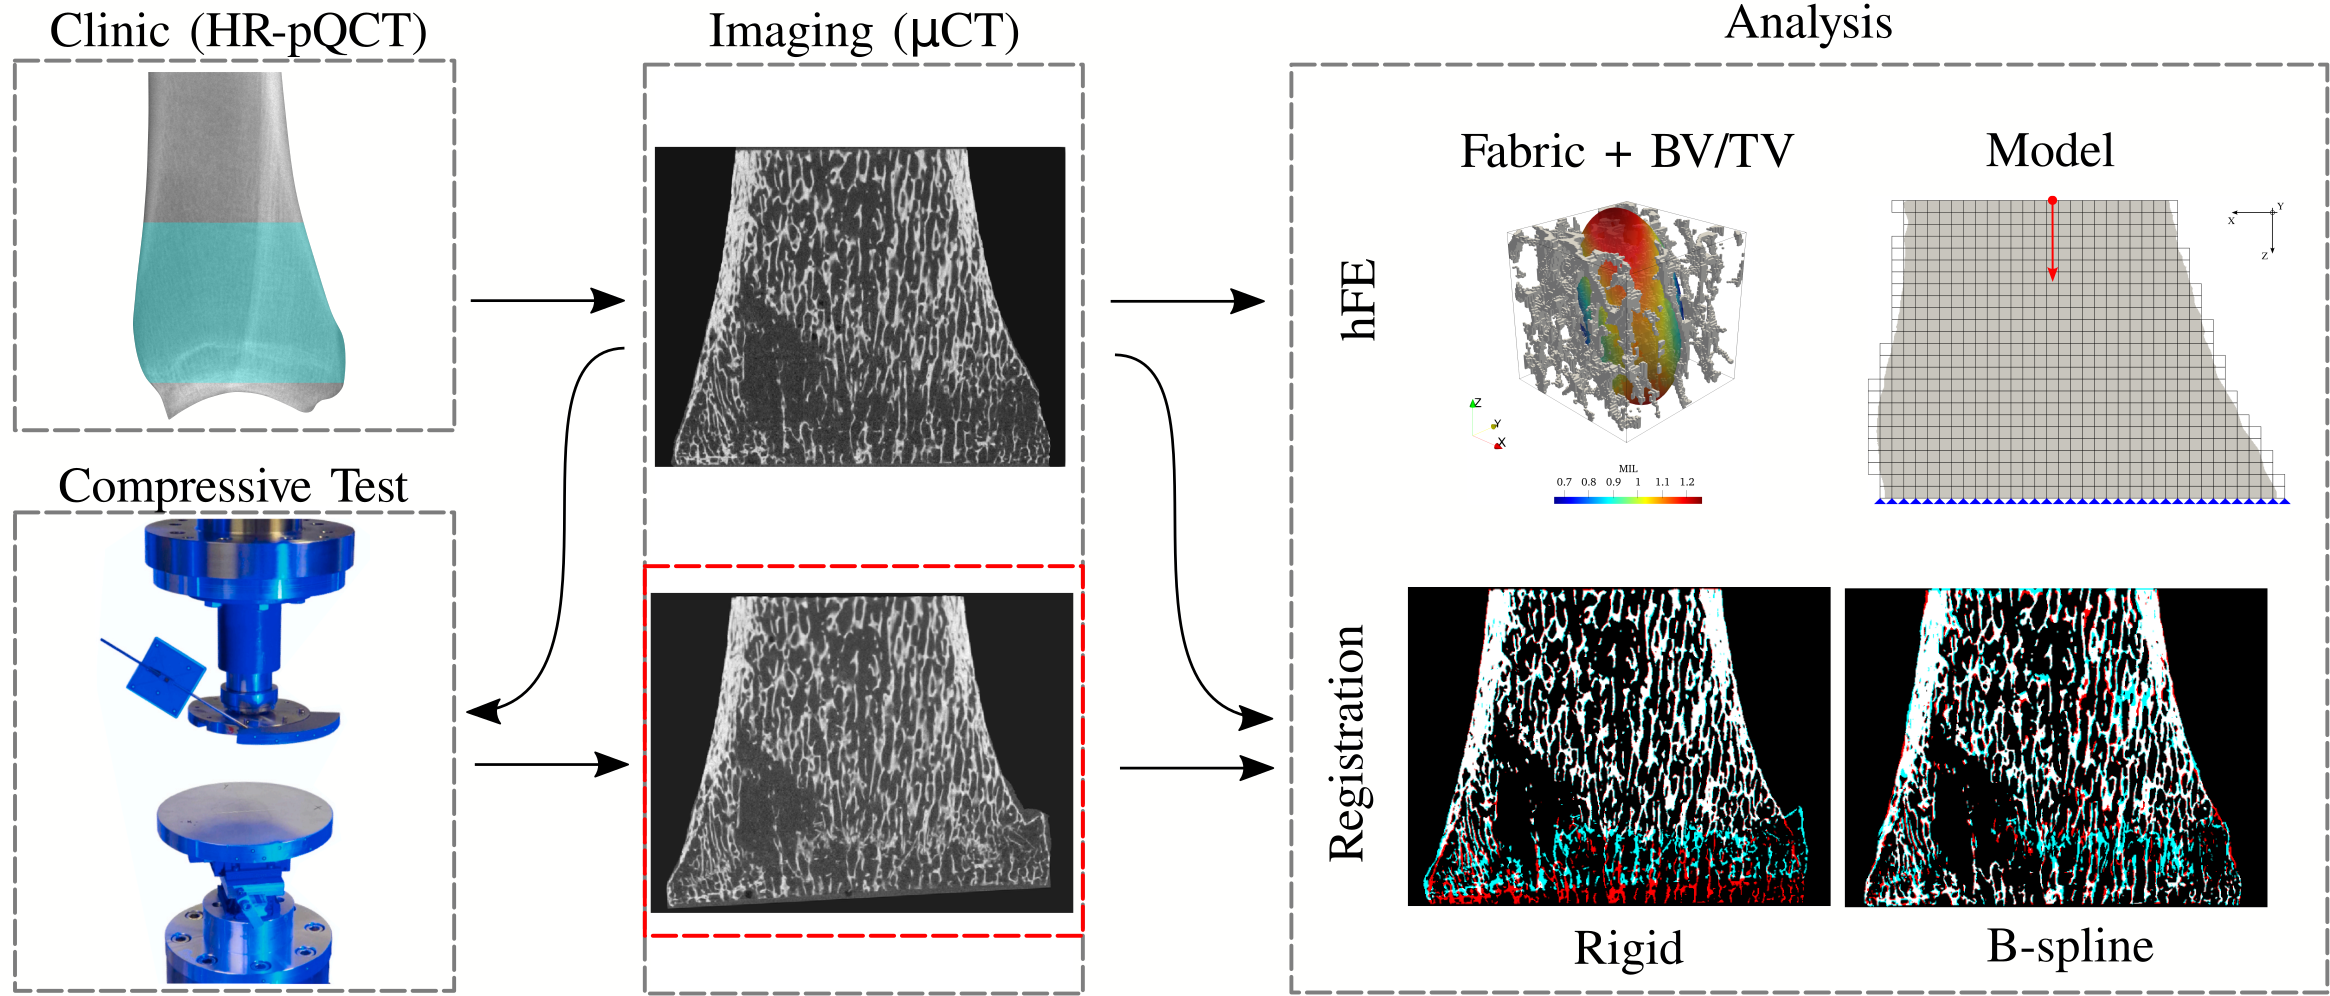
\includegraphics[width=1.0\linewidth]{Figures/Methods4}
	% \end{frame}

	% \begin{frame}[noframenumbering]
	% 	\frametitle{Pre- and Post-Test MicroCT Scans}
	% 	Digital Volume Correlation (DVC)
	% 	\vfill
	% 	\centering
	% 	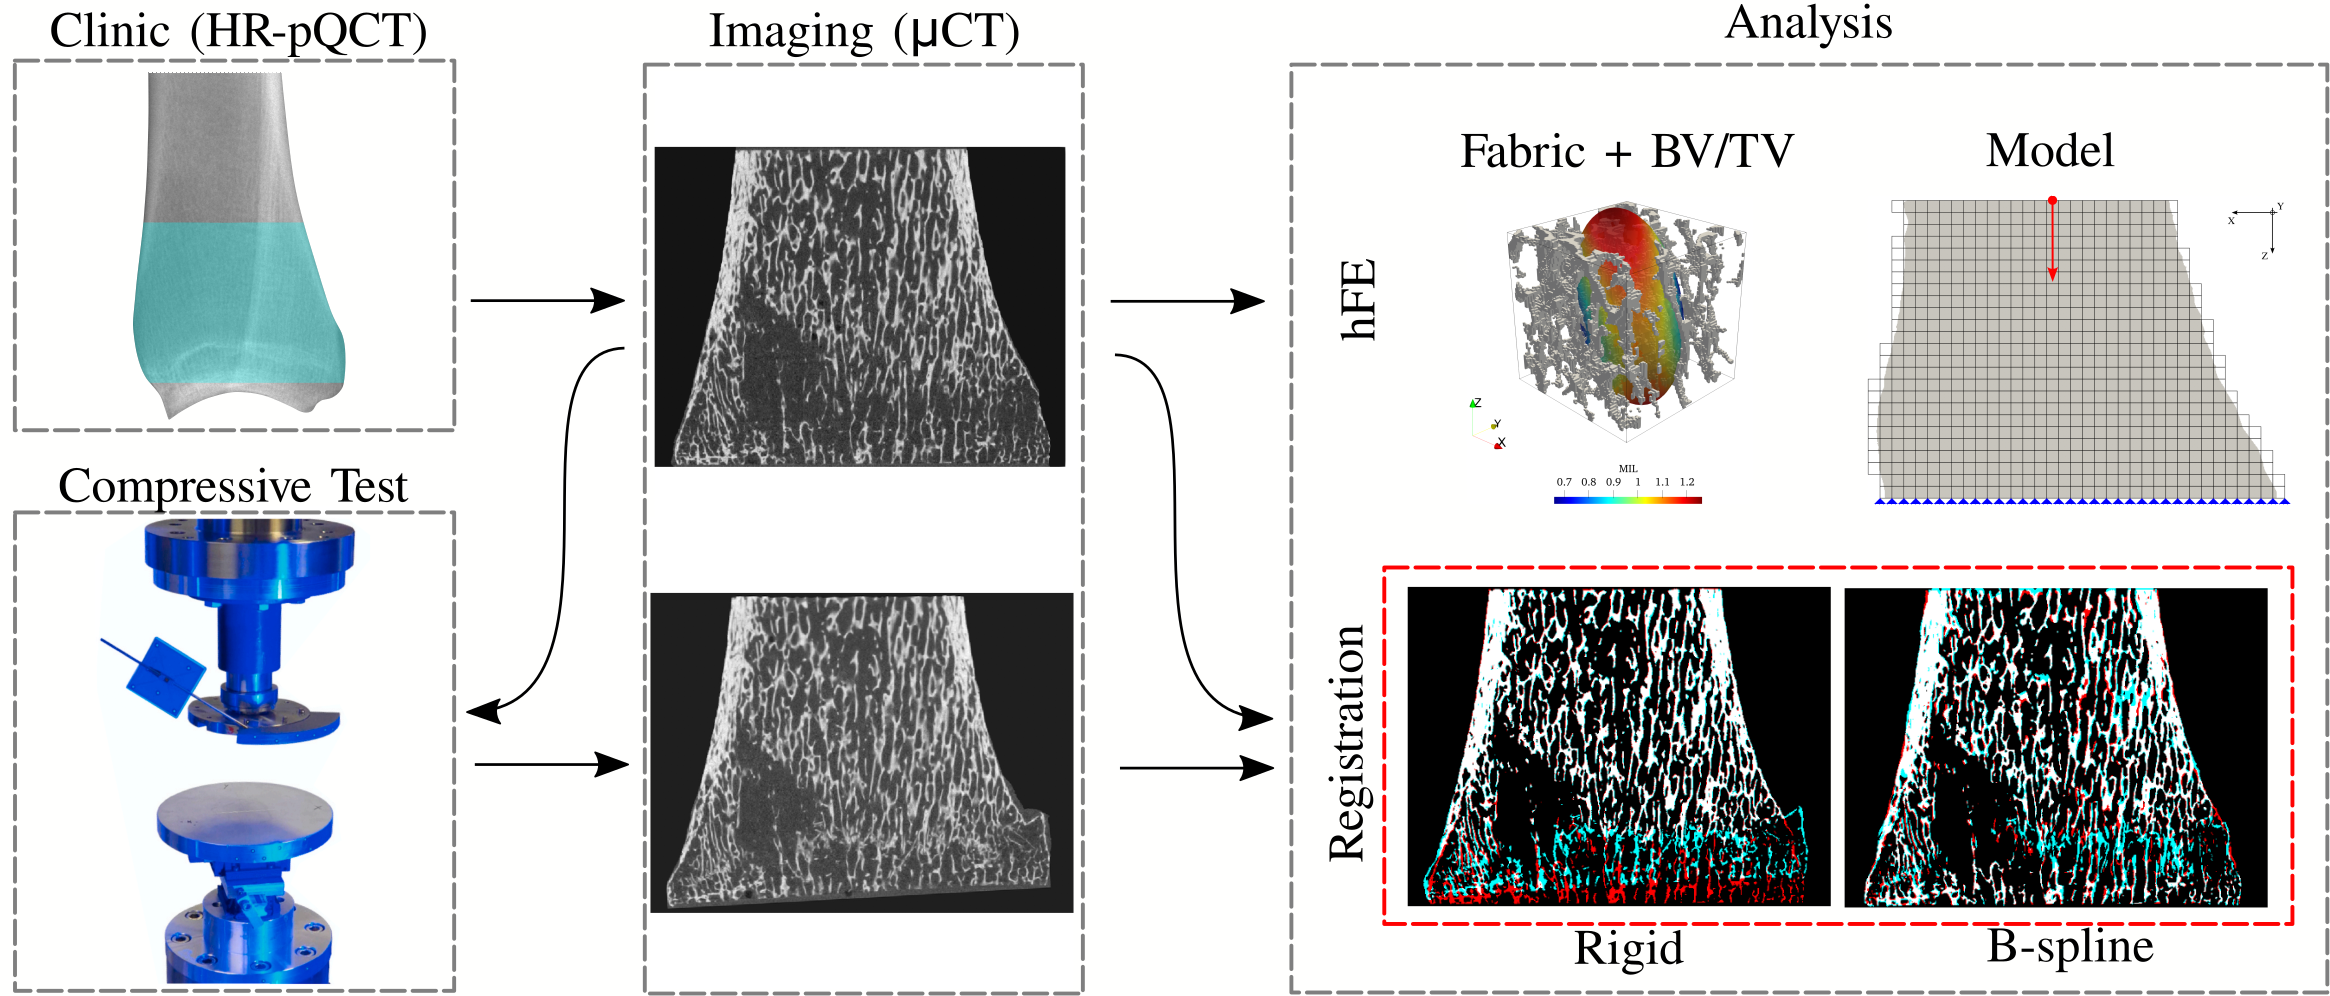
\includegraphics[width=1.0\linewidth]{Figures/Methods4b}
	% \end{frame}

	% \begin{frame}[noframenumbering]
	% 	\frametitle{Pre- and Post-Test MicroCT Scans}
	% 	Digital Volume Correlation (DVC)
	% 	\vfill
	% 	\centering
	% 	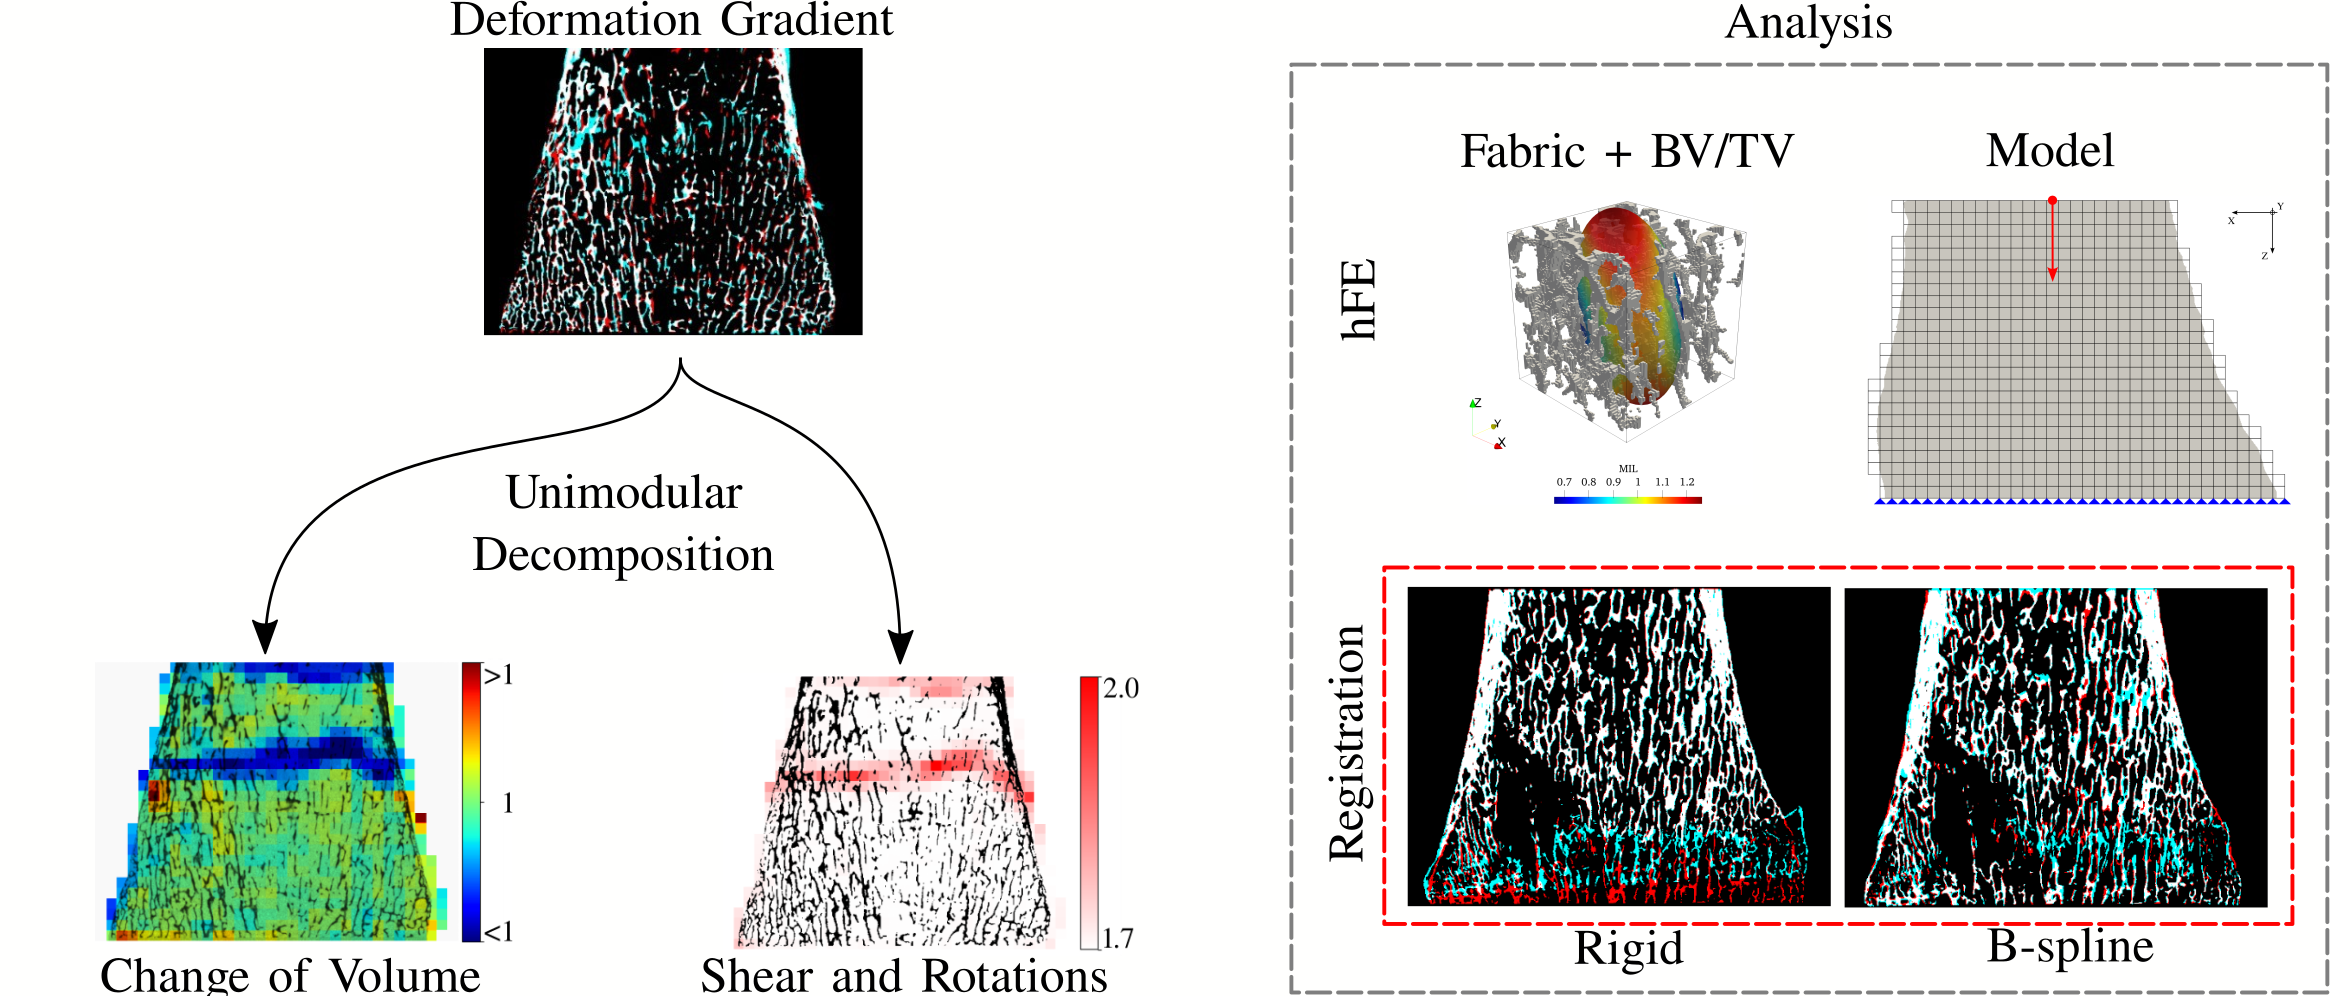
\includegraphics[width=1.0\linewidth]{Figures/Methods4d}
	% \end{frame}

	% \begin{frame}[noframenumbering]
	% 	\frametitle{HR-pQCT and MicroCT-based hFE}
	% 	Confirm similar results
	% 	\vfill
	% 	\centering
	% 	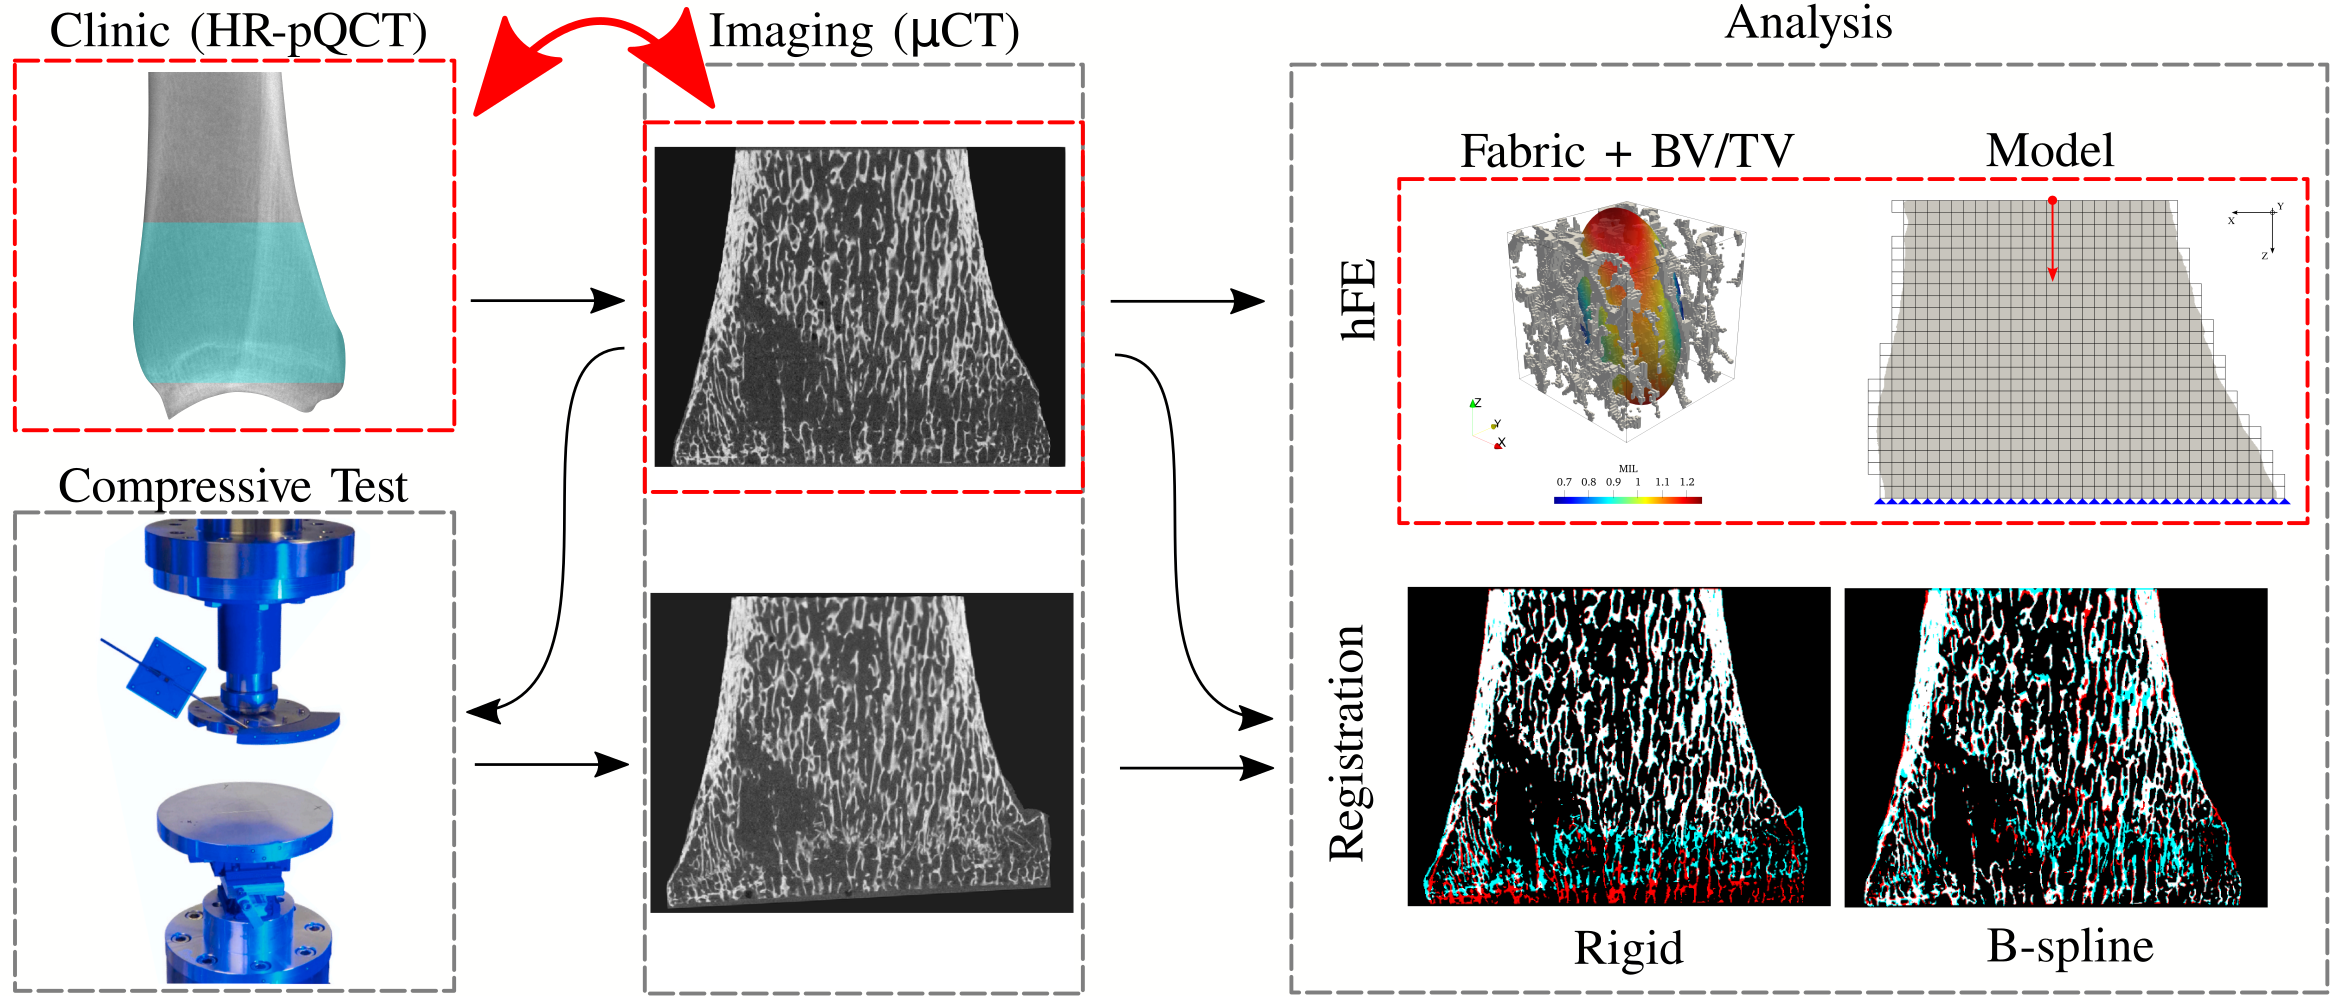
\includegraphics[width=1.0\linewidth]{Figures/Methods5b}
	% \end{frame}

	% \begin{frame}[noframenumbering]
	% 	\frametitle{Densitometry and Mechanics}
	% 	Confirm densitometry prediction capacity
	% 	\vfill
	% 	\centering
	% 	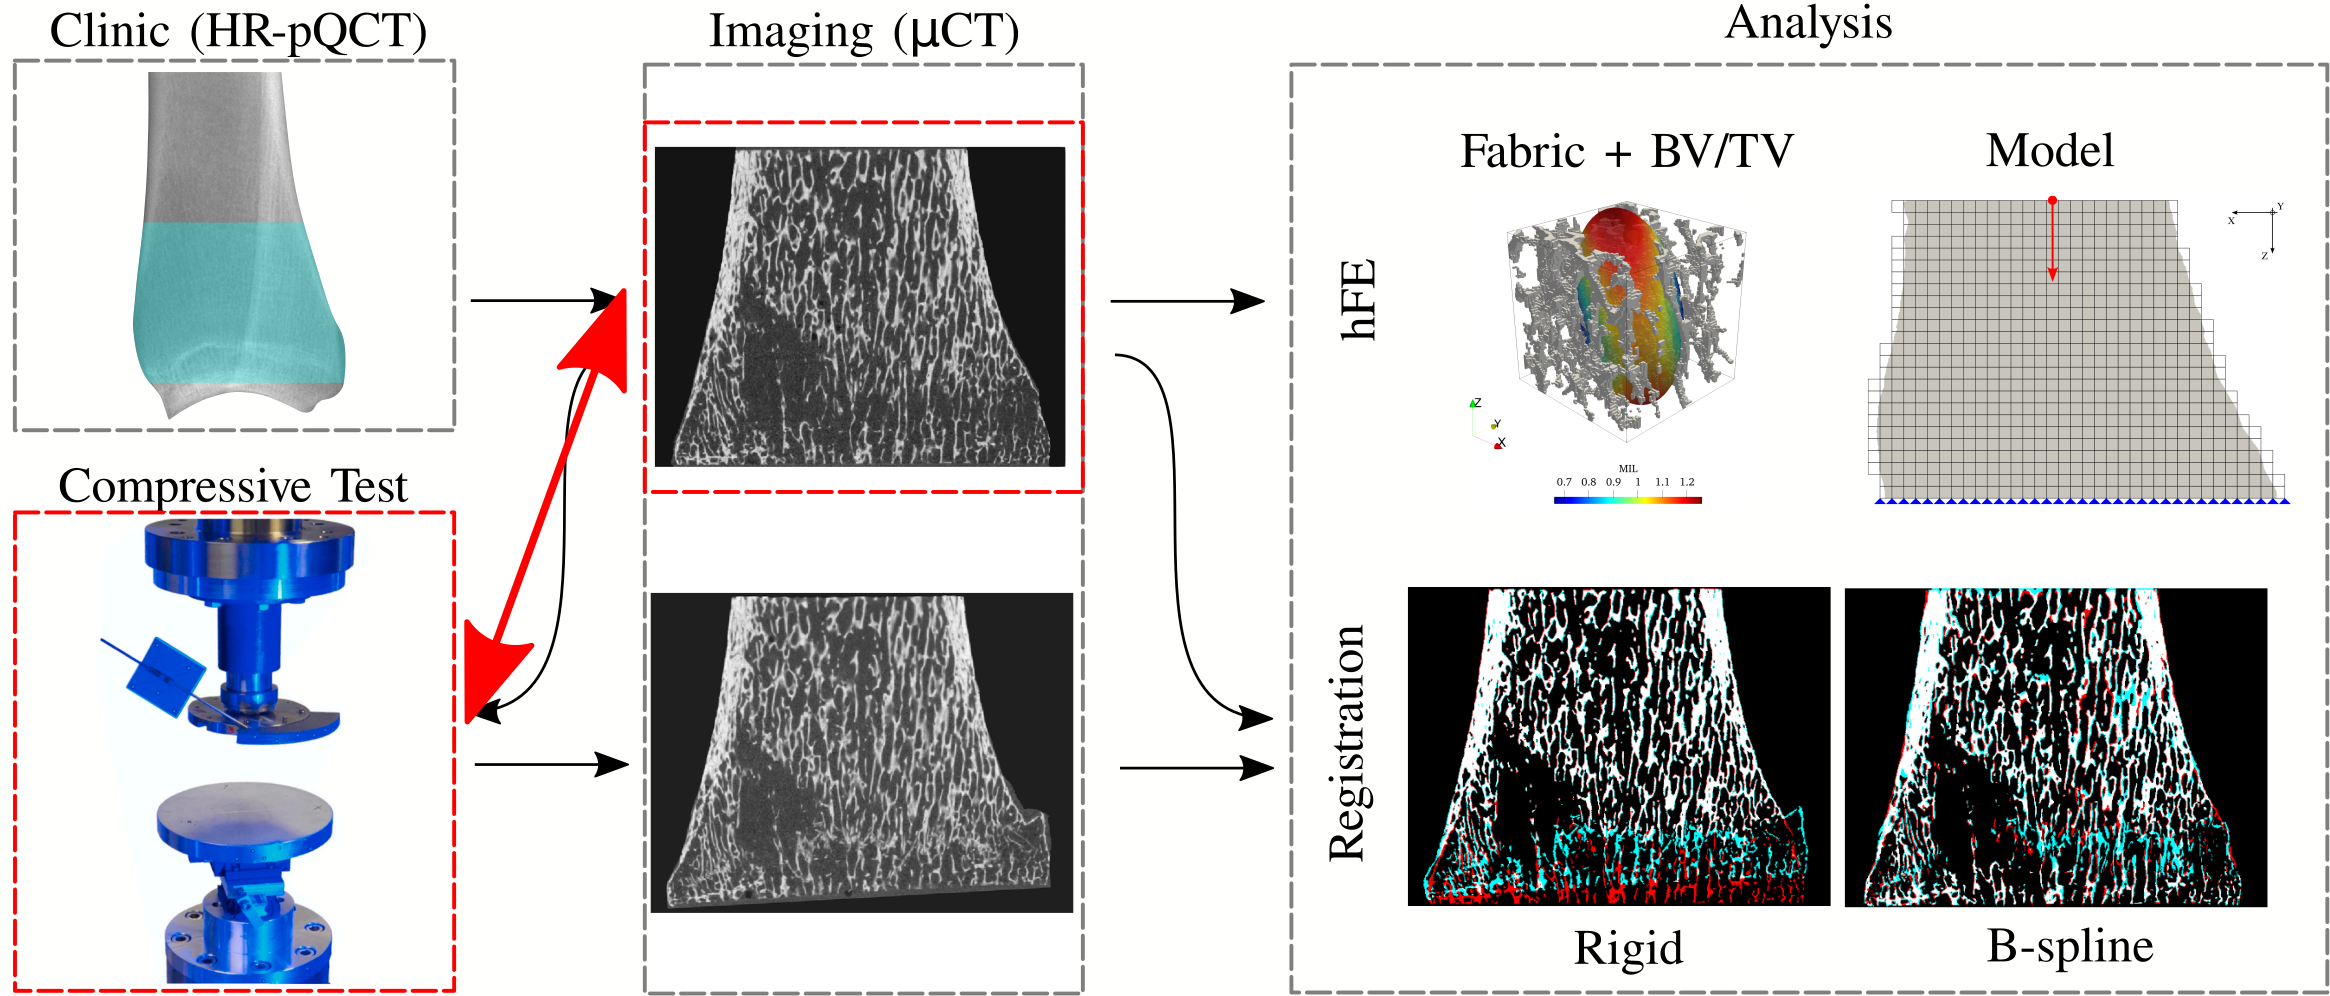
\includegraphics[width=1.0\linewidth]{Figures/Methods6}
	% \end{frame}

	% \begin{frame}[noframenumbering]
	% 	\frametitle{Structural Results}
	% 	Simulation validation by experiment
	% 	\vfill
	% 	\centering
	% 	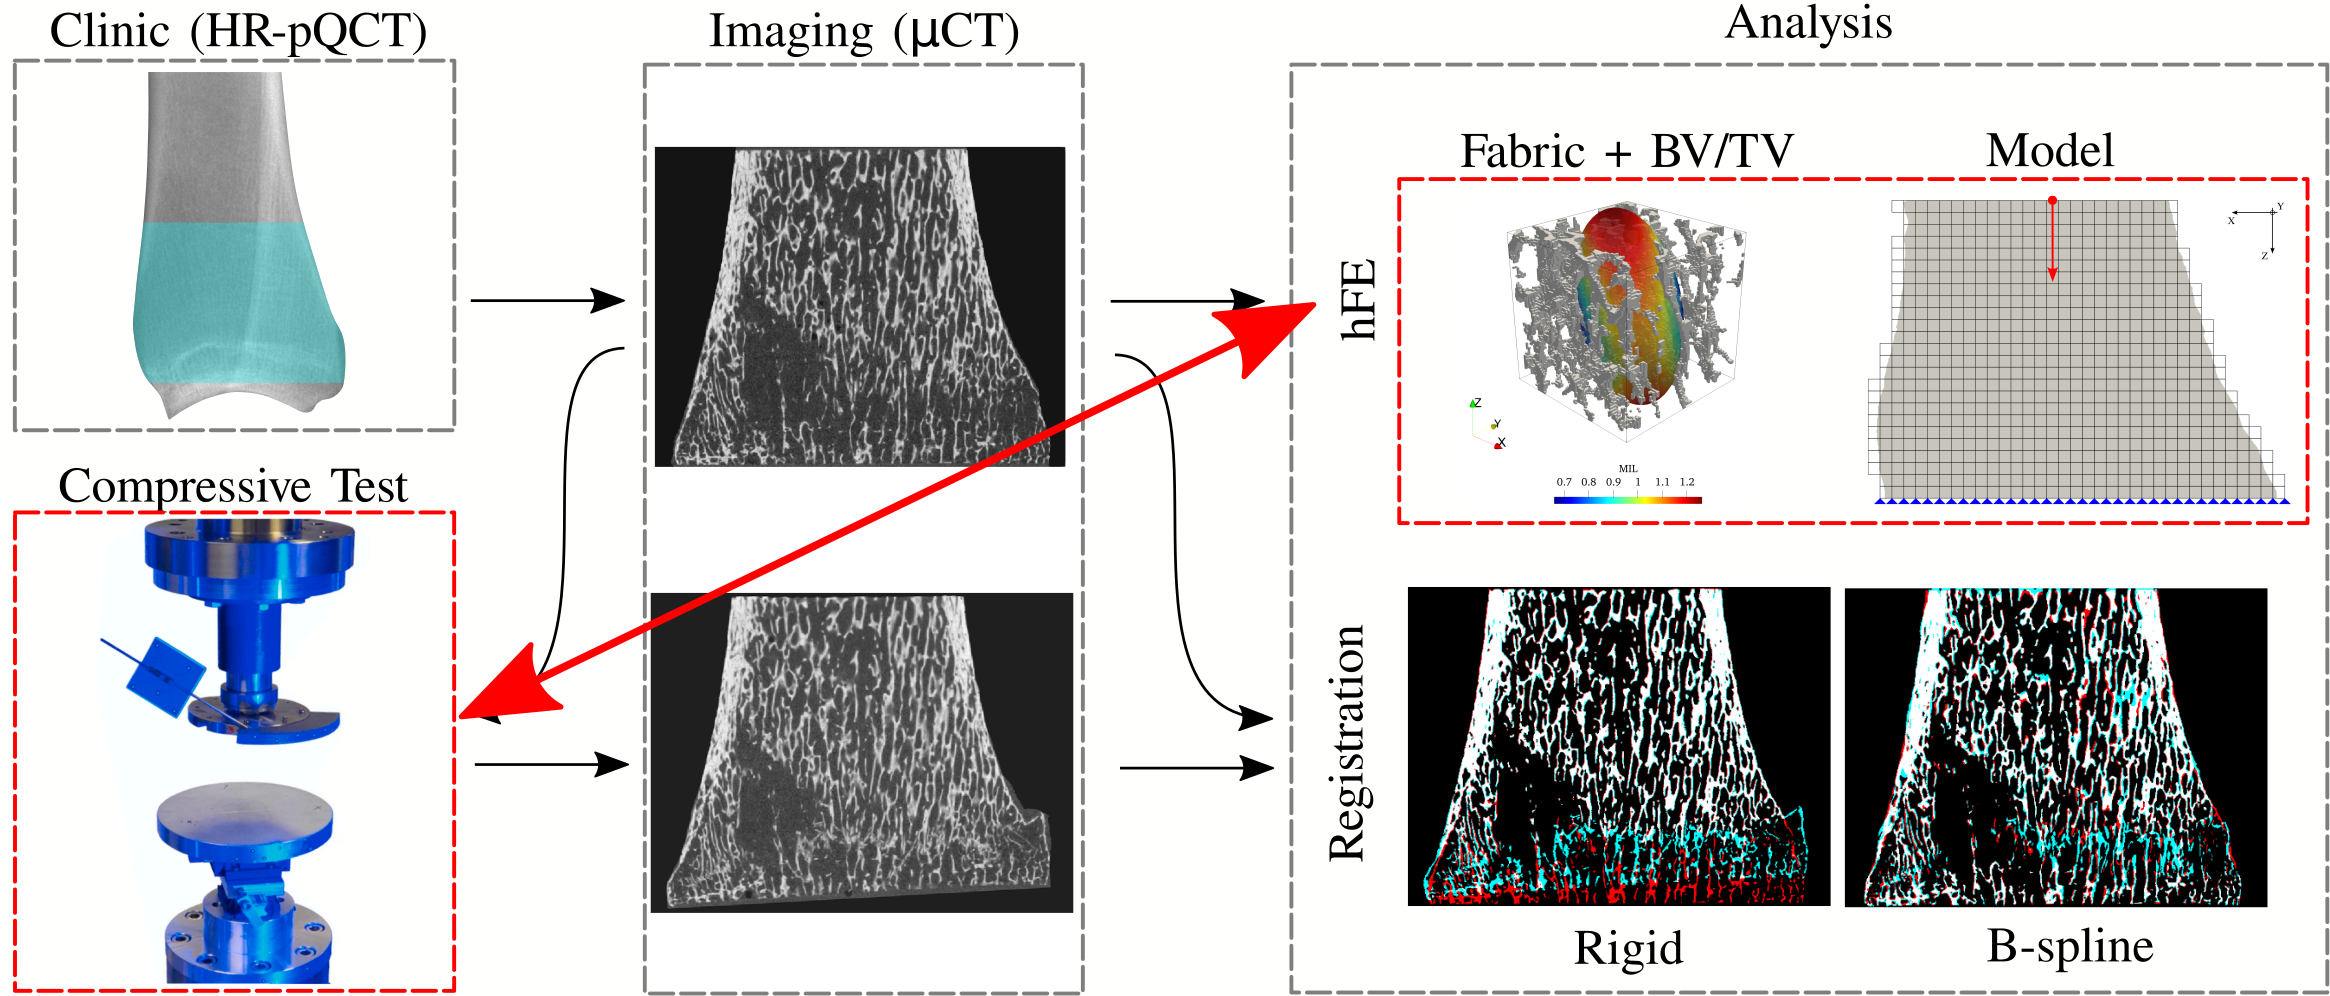
\includegraphics[width=1.0\linewidth]{Figures/Methods7}
	% \end{frame}

	% \begin{frame}[noframenumbering]
	% 	\frametitle{Strain Localization}
	% 	Simulation comparison with DVC
	% 	\vfill
	% 	\centering
	% 	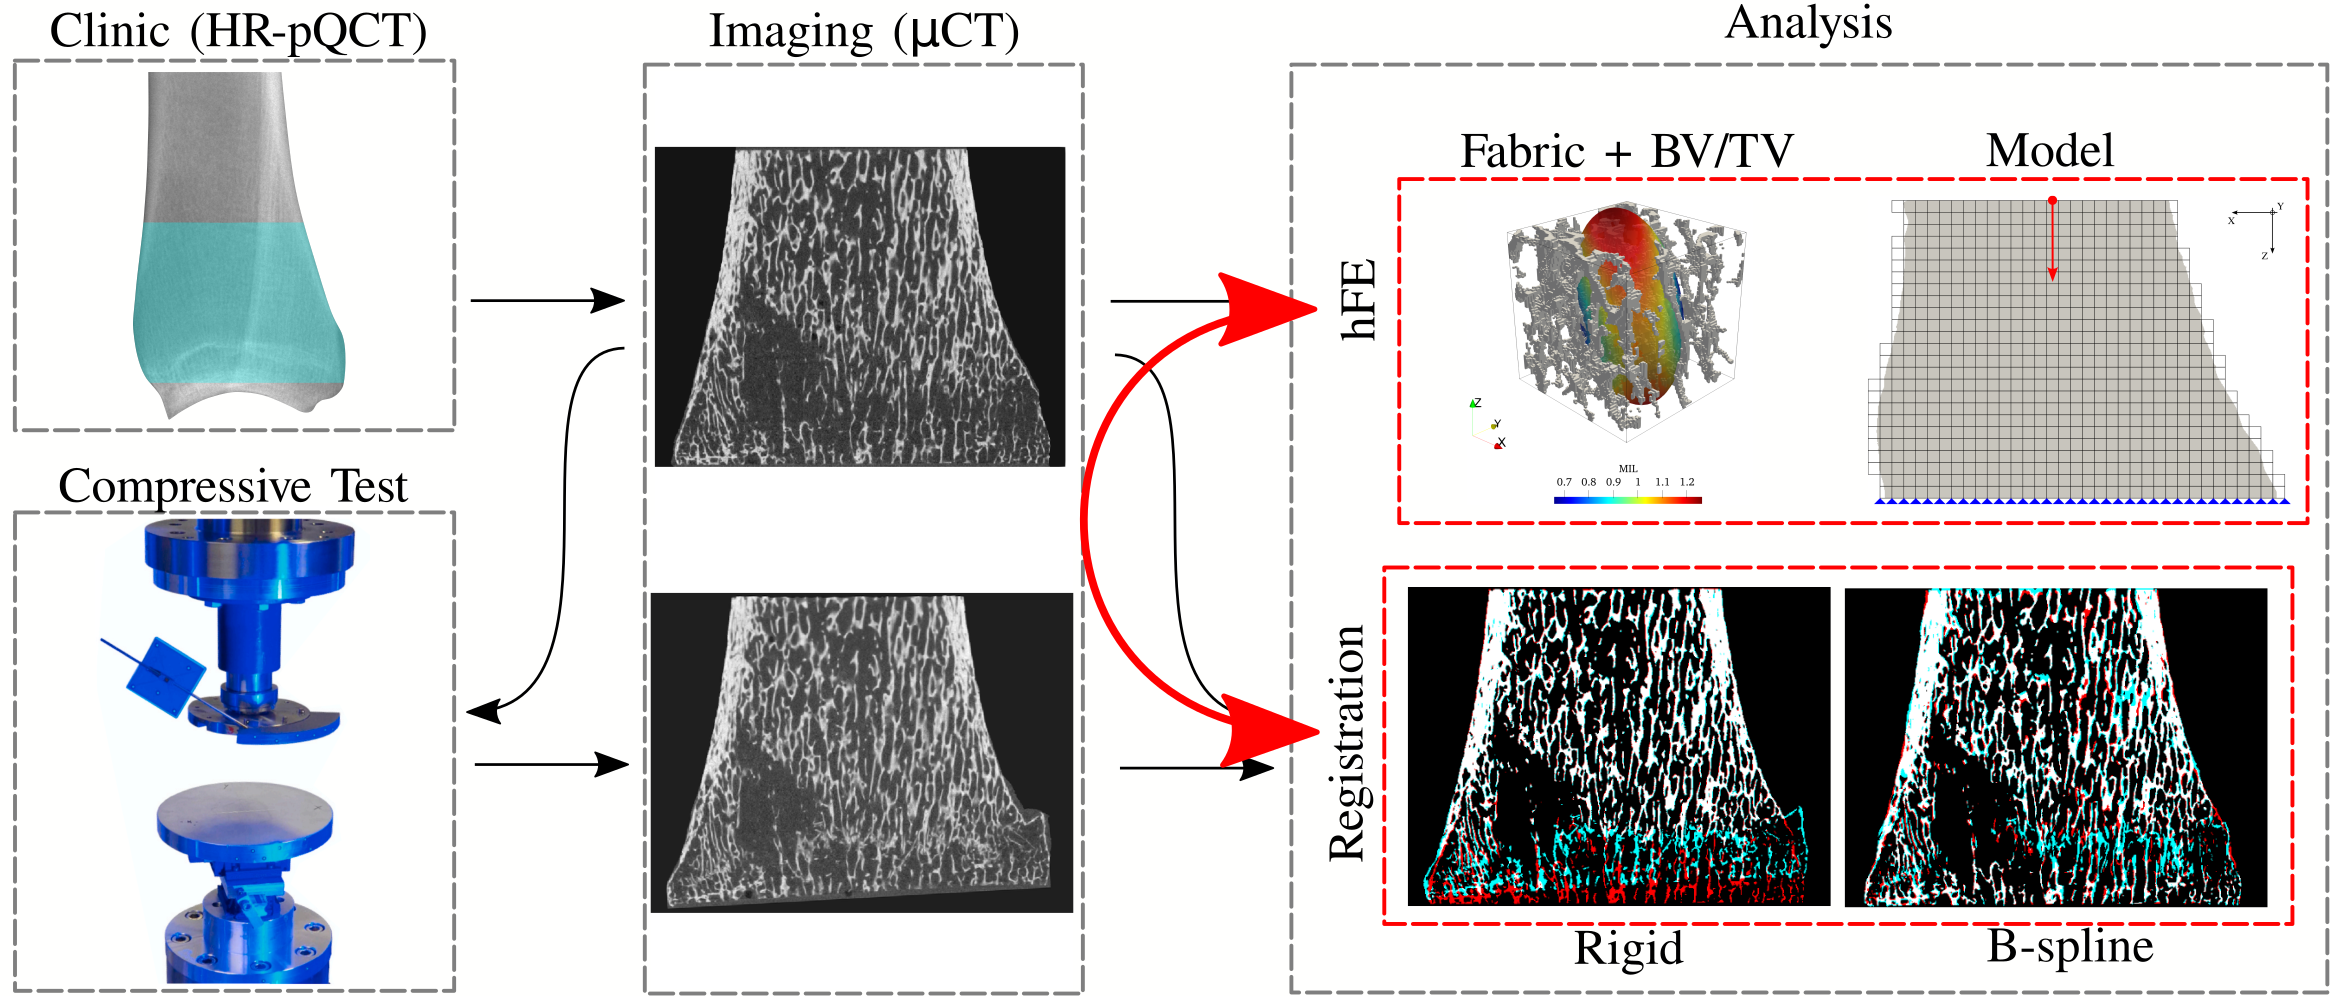
\includegraphics[width=1.0\linewidth]{Figures/Methods8}
	% \end{frame}

	%----------------------------------------------------------------
	%----------------------------------------------------------------
	%----------------------------------------------------------------
	
	\section{Results and Discussion}

	\begin{frame}
		\frametitle{Structural Variables}
		\begin{columns}
			\column[t]{0.3\linewidth}
			\centering
			\includegraphics[width=1.0\linewidth, trim=4 0 4 0]{Figures/HRpQCTvsMicroCT_Stiffness}\\
			HR-pQCT and \textmu CT
			\column[t]{0.3\linewidth}
			\centering
			\includegraphics[width=1.0\linewidth]{Figures/BMCvsStiffness}\\
			Densitometry and Experiment
			\column[t]{0.3\linewidth}
			\centering
			\includegraphics[width=1.0\linewidth]{Figures/hFEvsExp_Stiffness}\\
			Experiment and hFE
		\end{columns}
		\vspace{10mm}
		\centering
		$\Rightarrow$ Validation of hFE	for distal tibia
	\end{frame}

	% \begin{frame}
	% 	\frametitle{HR-pQCT and \textmu CT}
	% 	\begin{columns}
	% 		\column{0.5\linewidth}
	% 		\vfill
	% 		\begin{itemize}
	% 			\item Very high correlation\vspace{0.75cm}
	% 			\item Slope CI comprises 1\vspace{0.75cm}
	% 			\item Not exactly the same structure\vspace{0.75cm}
	% 		\end{itemize}
	% 		\vfill
	% 		\column{0.5\linewidth}
	% 		\centering
	% 		\includegraphics[width=1.0\linewidth]{Pictures/HRpQCTvsMicroCT_Stiffness}
	% 	\end{columns}
	% \end{frame}

	% \begin{frame}
	% 	\frametitle{Densitometry and Experiment}
	% 	\begin{columns}
	% 		\column{0.5\linewidth}
	% 		\vfill
	% 		\begin{itemize}
	% 			\item High correlation\vspace{0.75cm}
	% 			\item Outlier\vspace{0.75cm}
	% 			\item No structural information\vspace{0.75cm}
	% 		\end{itemize}
	% 		\vfill
	% 		\column{0.5\linewidth}
	% 		\centering
	% 		\includegraphics[width=1.0\linewidth]{Pictures/BMCvsStiffness}
	% 	\end{columns}
	% \end{frame}

	% \begin{frame}
	% 	\frametitle{Experiment and hFE}
	% 	\begin{columns}
	% 		\column{0.5\linewidth}
	% 		\vfill
	% 		\begin{itemize}
	% 			\item 3D structure\vspace{0.6cm}
	% 			\item No outlier\vspace{0.6cm}
	% 			\item Slope CI comprises 1\vspace{0.6cm}
	% 		\end{itemize}
	% 		$\Rightarrow$ hFE validation by experiment\vspace{0.7cm}\\
	% 		\vfill
	% 		\column{0.5\linewidth}
	% 		\centering
	% 		\includegraphics[width=1.0\linewidth]{Pictures/hFEvsExp_Stiffness}
	% 	\end{columns}
	% \end{frame}

	\begin{frame}
		\frametitle{Field Variables}
		\framesubtitle{Strain Localization}
		\begin{columns}
			\column{0.6\linewidth}
			Only 2 good agreement (8\%)
				\begin{itemize}
					\item Boundary conditions
					\item No morphological mesh
				\end{itemize}

			\column{0.35\linewidth}		
				$\Rightarrow$ Limitation of hFE	
		\end{columns}

		\vspace{0.5cm}
		\centering
		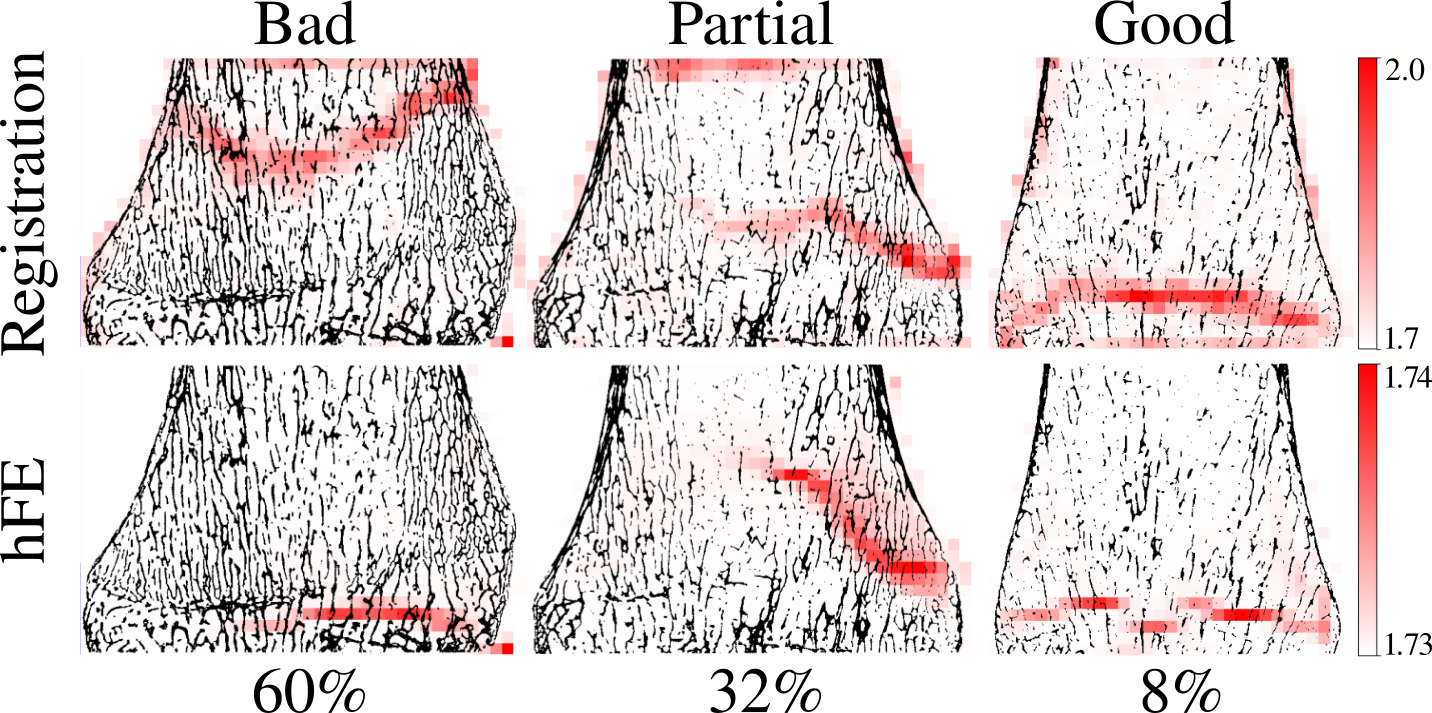
\includegraphics[width=0.8\linewidth]{Figures/Comparison}
	\end{frame}

	%----------------------------------------------------------------
	%----------------------------------------------------------------
	%----------------------------------------------------------------
	
	\section{Conclusions}
	
	\begin{frame}
		\frametitle{Conclusions}

		Mechanical Experiment
		\begin{itemize}
			\item First data set on distal tibia sections
		\end{itemize}

		\vspace{0.25cm}

		Densitometry
		\begin{itemize}
			\item High correlation with mechanical properties
			\item Outliers
		\end{itemize}

		\vspace{0.25cm}

		Homogenized Finite Elements
		\begin{itemize}
			\item 3D structural information remove outliers
			\item Validated by experiment for distal tibia\\
				  $\Rightarrow$ Up to ultimate load
			\item Limited capacity for strain localization prediction\\
			      $\Rightarrow$ Boundary conditions and meshing strategy
		\end{itemize}

	\end{frame}
	
	%----------------------------------------------------------------
	%----------------------------------------------------------------
	%----------------------------------------------------------------
	
	\section{}
	\begin{frame}
		\frametitle{Acknowledgements}
		Funds:
		\begin{itemize}
			\item ARTORG Center for Biomedical Engineering Research
		\end{itemize}
		\vspace{5mm}

		\begin{columns}
			\column{0.65\linewidth}
			Samples
			\begin{itemize}
				\item Division of Anatomy\\Center for Anatomy and Cell Biology\\Medical University of Vienna\\Vienna, Austria
			\end{itemize}
			\vspace{5mm}
			Compression testing
			\begin{itemize}
				\item AO Research Institute Davos\\7270 Davos, Switzerland
			\end{itemize}

			\column{0.25\linewidth}
			\centering
			\vfill
			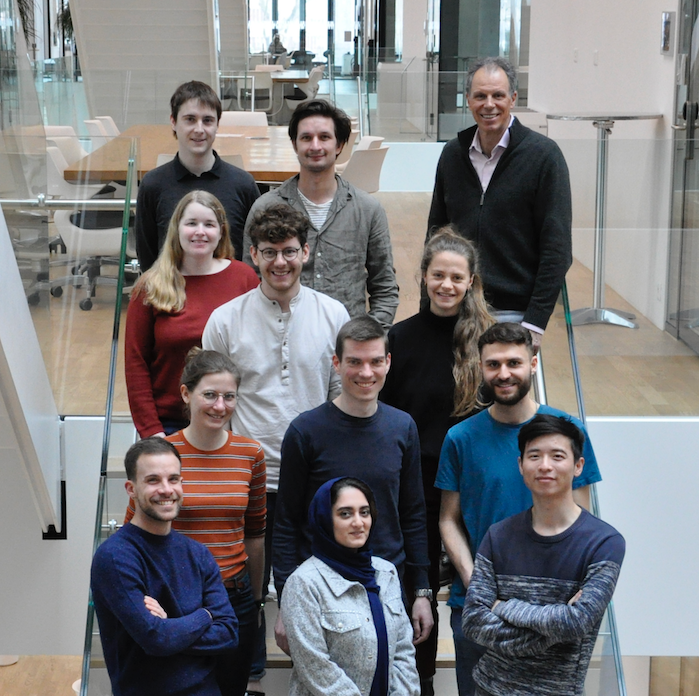
\includegraphics[width=1.0\linewidth, trim=40 0 0 0]{Figures/GroupPhoto}

		\end{columns}

	\end{frame}

	\begin{frame}
		\frametitle{Digital Volume Correlation}
		\framesubtitle{Elastix}
		Open-source software for image registration
		\begin{itemize}
			\item Metrics: Mean Squared Difference, Normalised Correlation Coefficient, Mutual Information, Kappa Statistic
			\item Samplers: Full, Grid, Random, Random Coordinate
			\item Interpolators: Nearest Neighbour, Linear, N-th order BSpline
			\item Transforms: Translation, Rigid, Similarity, Affine, BSplines
			\item Optimisers: Gradient descent, Robbins-Monro
			\item Multi-resolution: Gaussian pyramid, Gaussian scale space, Shrinking pyramid
		\end{itemize}
		\vfill
		$\Rightarrow$ Available as a library in C++, Python, R, Java, Ruby, and Lua
	\end{frame}

	\begin{frame}
		\frametitle{Elastix}
		\framesubtitle{Manual}
		\begin{columns}
			\column{0.4\linewidth}
			Outline
			\begin{itemize}
				\item Introduction
				\item Registration
				\item Elastix
				\item Transformix
				\item Tutorial
				\item Advanced Topics
				\item Developers Guide
			\end{itemize}

			\column{0.5\linewidth}
			 \centering
			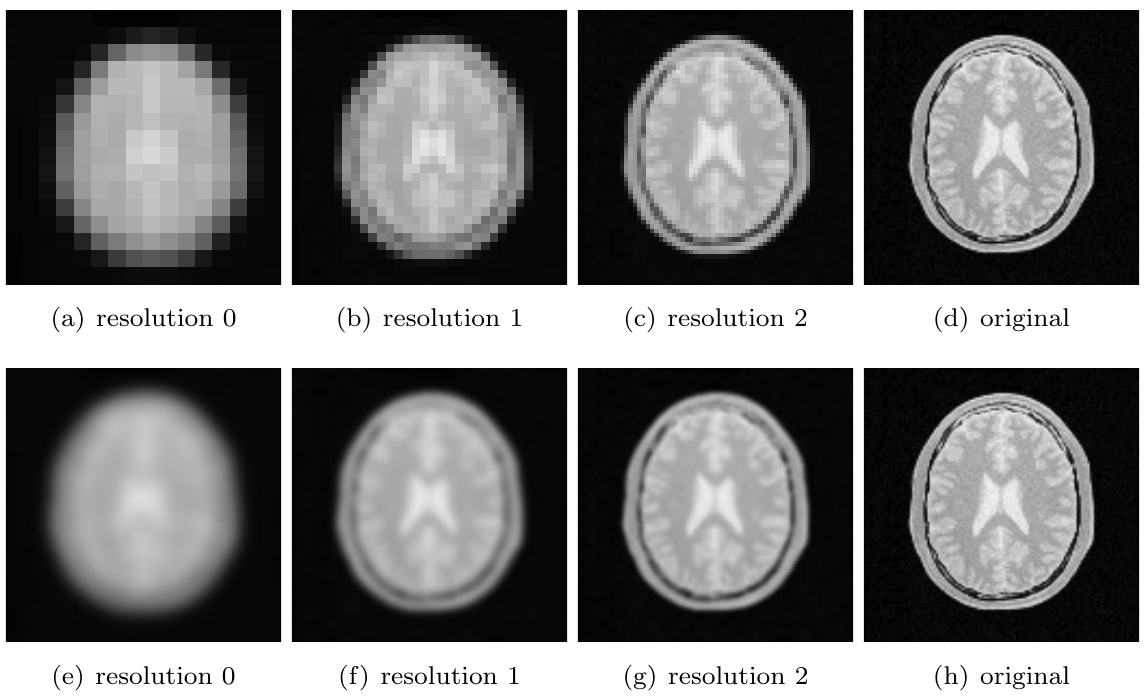
\includegraphics[width=0.8\linewidth]{Figures/Elastix1.png}\\
			\vfill
			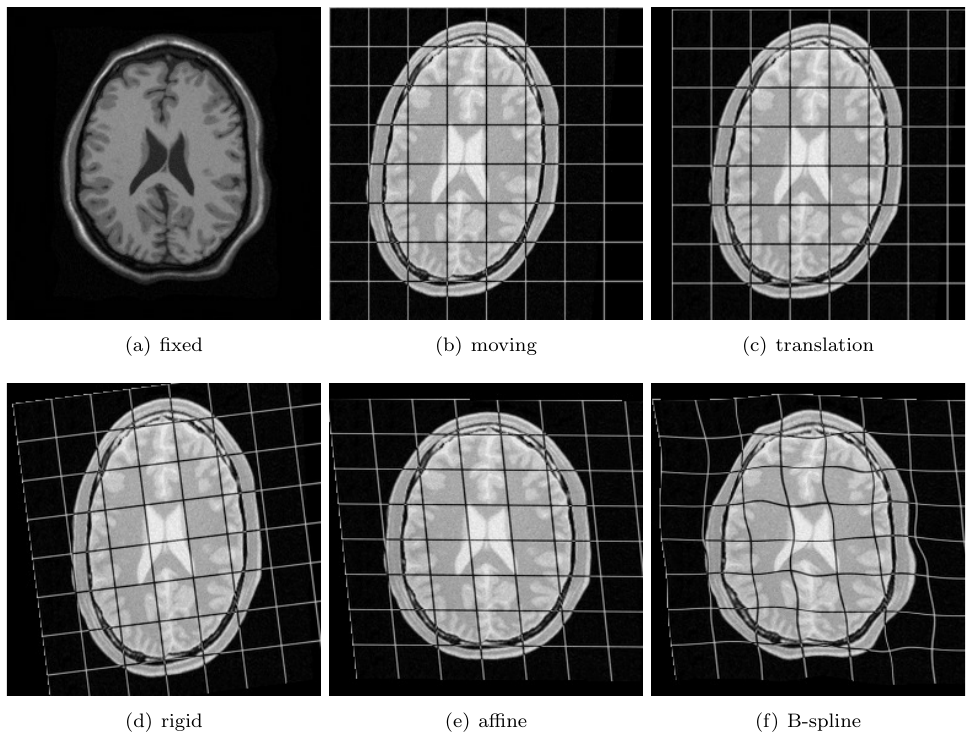
\includegraphics[width=0.8\linewidth]{Figures/Elastix2.png}
		\end{columns}
	\end{frame}
	
	%----------------------------------------------------------------
	%----------------------------------------------------------------
	%----------------------------------------------------------------
	
	\appendix
	
	\section{Appendix}

	\begin{frame}
		\frametitle{Strain Localization}
		Unimodular decomposition: $\mathbf{F} = \det(\mathbf{F})^{-1/3}\tilde{\mathbf{F}}$
		
		\vfill

		\begin{columns}
			\column{0.3\linewidth}
			\centering
			$\mathbf{F}$\\
			\vfill
			Def. gradient\\
			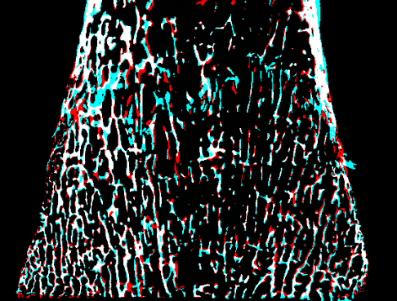
\includegraphics[width=\linewidth]{Figures/SL1}\\

			\column{0.33\linewidth}
			\centering
			$\det(\mathbf{F})$\\
			\vfill
			Change of volume\\
			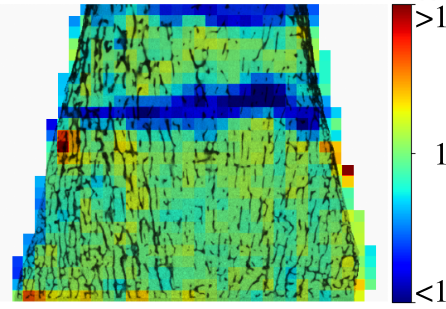
\includegraphics[width=\linewidth]{Figures/SL2}\\

			\column{0.33\linewidth}
			\centering
			$||\tilde{\mathbf{F}}||$\\
			\vfill
			Shear and rotations\\
			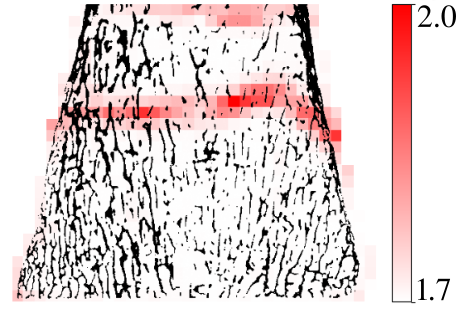
\includegraphics[width=\linewidth]{Figures/SL3}\\

		\end{columns}
	\end{frame}
	
	%----------------------------------------------------------------
	%----------------------------------------------------------------
	%----------------------------------------------------------------
	
\end{document}